% Appendix A

\chapter{Background additional material (search for long-lived HNL)} \label{AppendixA} 

\section{Estimation of single-fake background}\label{app:sfr}

Measuring the fake rate in jet events in data, we should take into
account the contamination of prompt leptons, mostly from $\PW$ and
$\PZ$ production in association with hadronic jets. To discriminate
between QCD and \PW events, we can use the transverse mass of the
lepton and the missing transverse momentum in the event, \MT.
The requirements on the maximum $\ptmiss$ and $\MT$ values
strongly reduce the contribution from prompt leptons in the
measurement region.
The residual contamination is subtracted both in the numerator and
denominator \ptc bins using simulated $\PW+\mathrm{jets}$, DY, and
\ttbar event from MC samples. The simulation is normalized in the
control region dominated by the \PW~$+$~jets and DY processes, with
$\ptmiss>20\GeV$ and $70<\MT<120\GeV$.
Due to different trigger pre-scales of the single-lepton trigger
listed in Table~\ref{tab:ctrlTriggers}, the MC normalization and the
subtraction of the contribution from prompt leptons are performed
separately for all triggers in the corresponding \pt ranges.

Figures~\ref{fig:sFR_mc} and \ref{fig:sFR_data} show the measured
values of \sfr for electrons and muons in simulation and in data,
respectively, as a function of \ptc and in different \abseta bins.
Figure~\ref{fig:sFR_mc} also shows that the contributions to \sfr from
light-quark and heavy-quark hadrons in simulation are comparable,
which is a necessary requirement in order to apply \sfr independently
of the flavor composition in the application region.
\begin{figure}[t!]
  \centering
  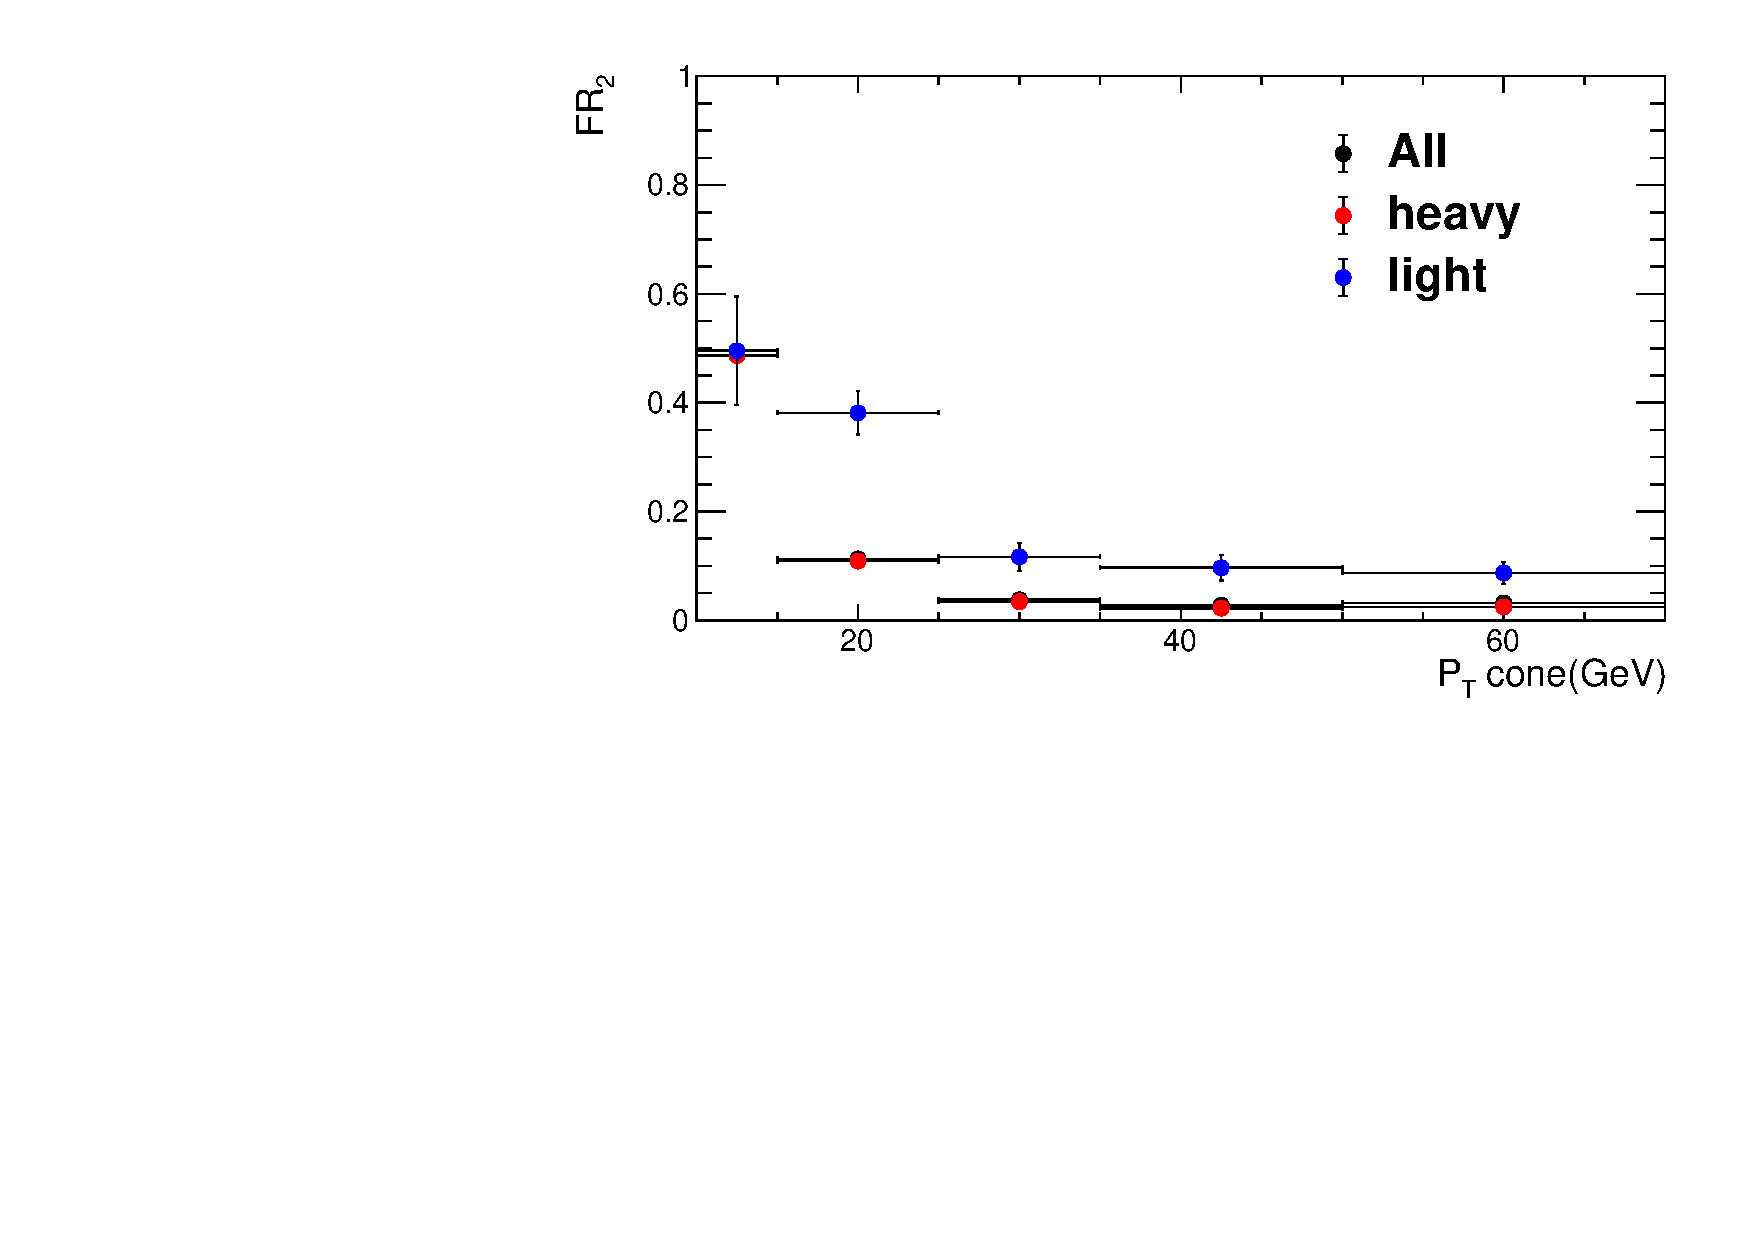
\includegraphics[width=.48\textwidth]{Figures/c6/backgrounds/FR/sFR/QCD/LeptonPt_ele_eta1_FR2.pdf}
  \hfill{}
  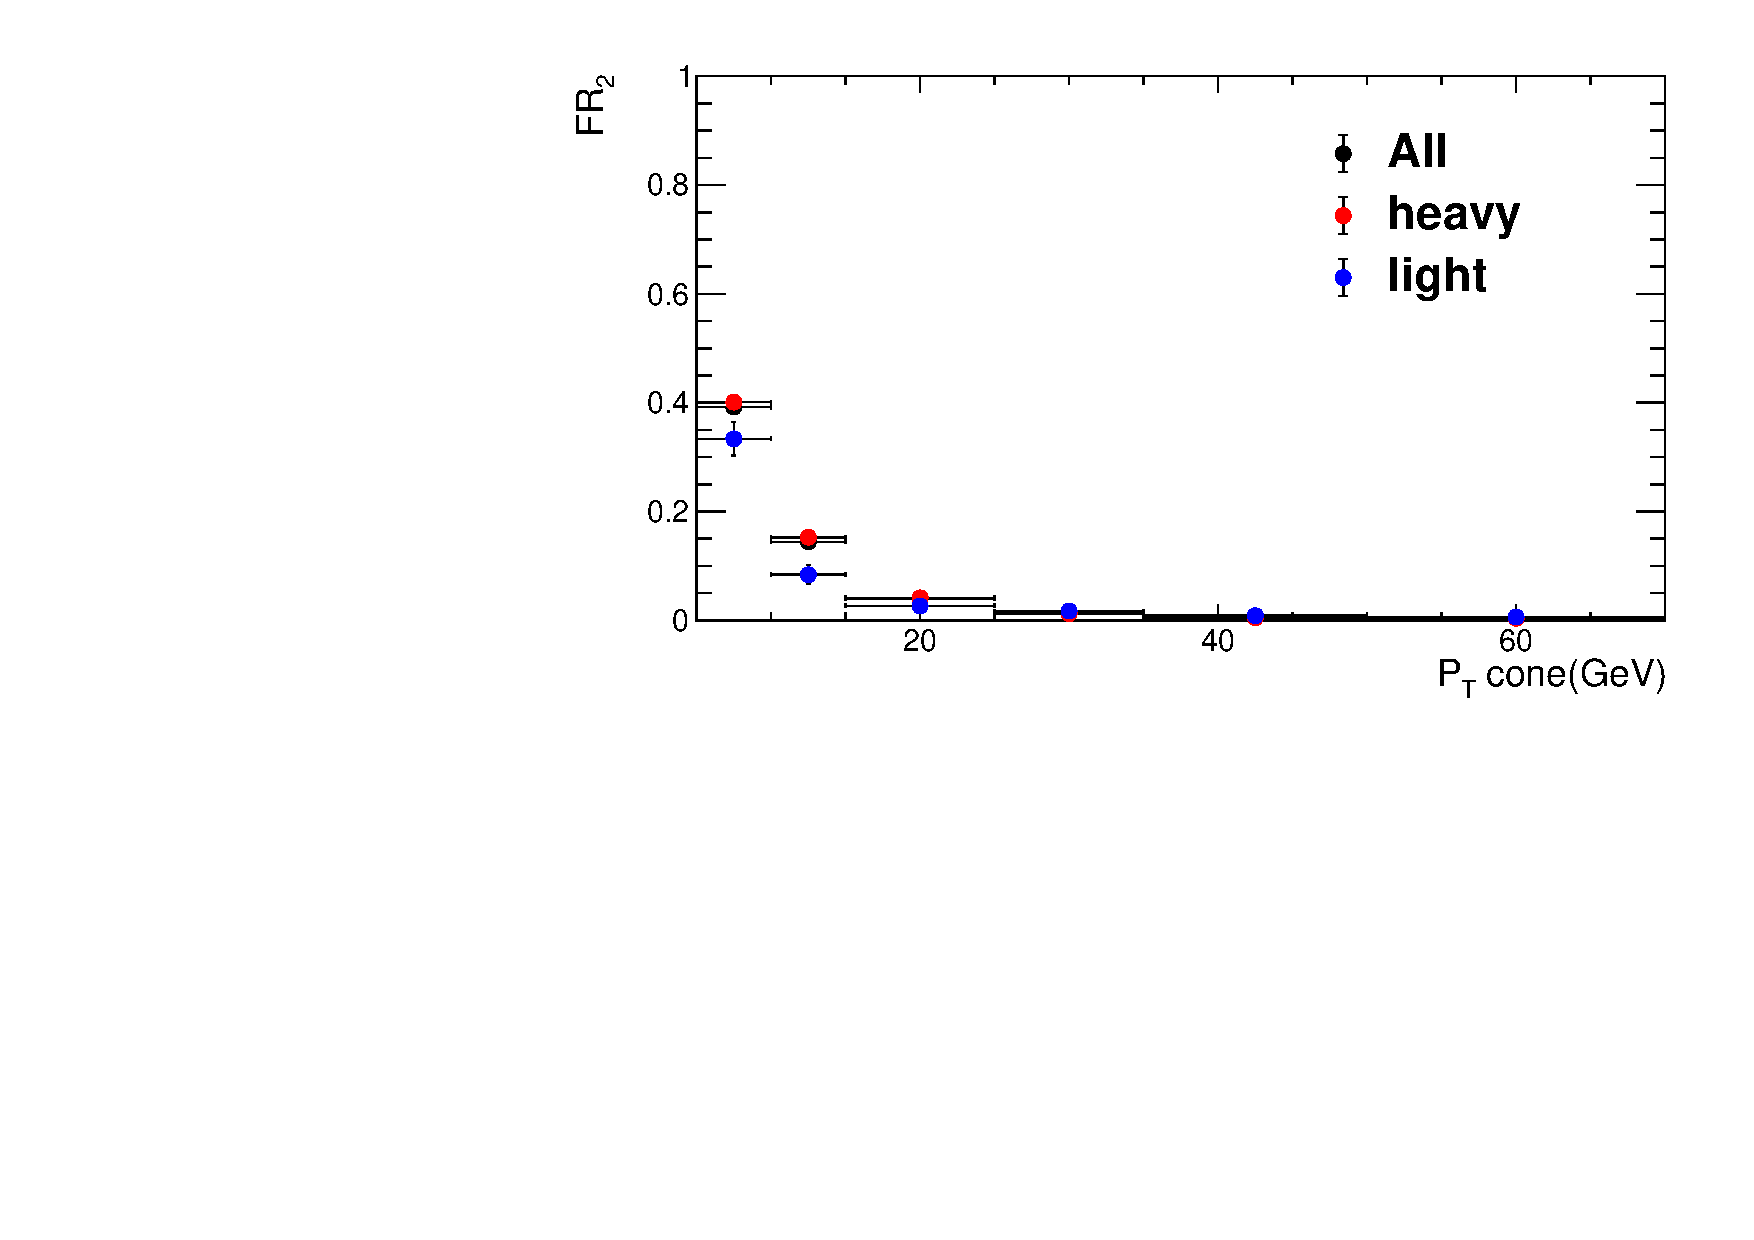
\includegraphics[width=.48\textwidth]{Figures/c6/backgrounds/FR/sFR/QCD/LeptonPt_mu_eta1_FR2.pdf}\\
  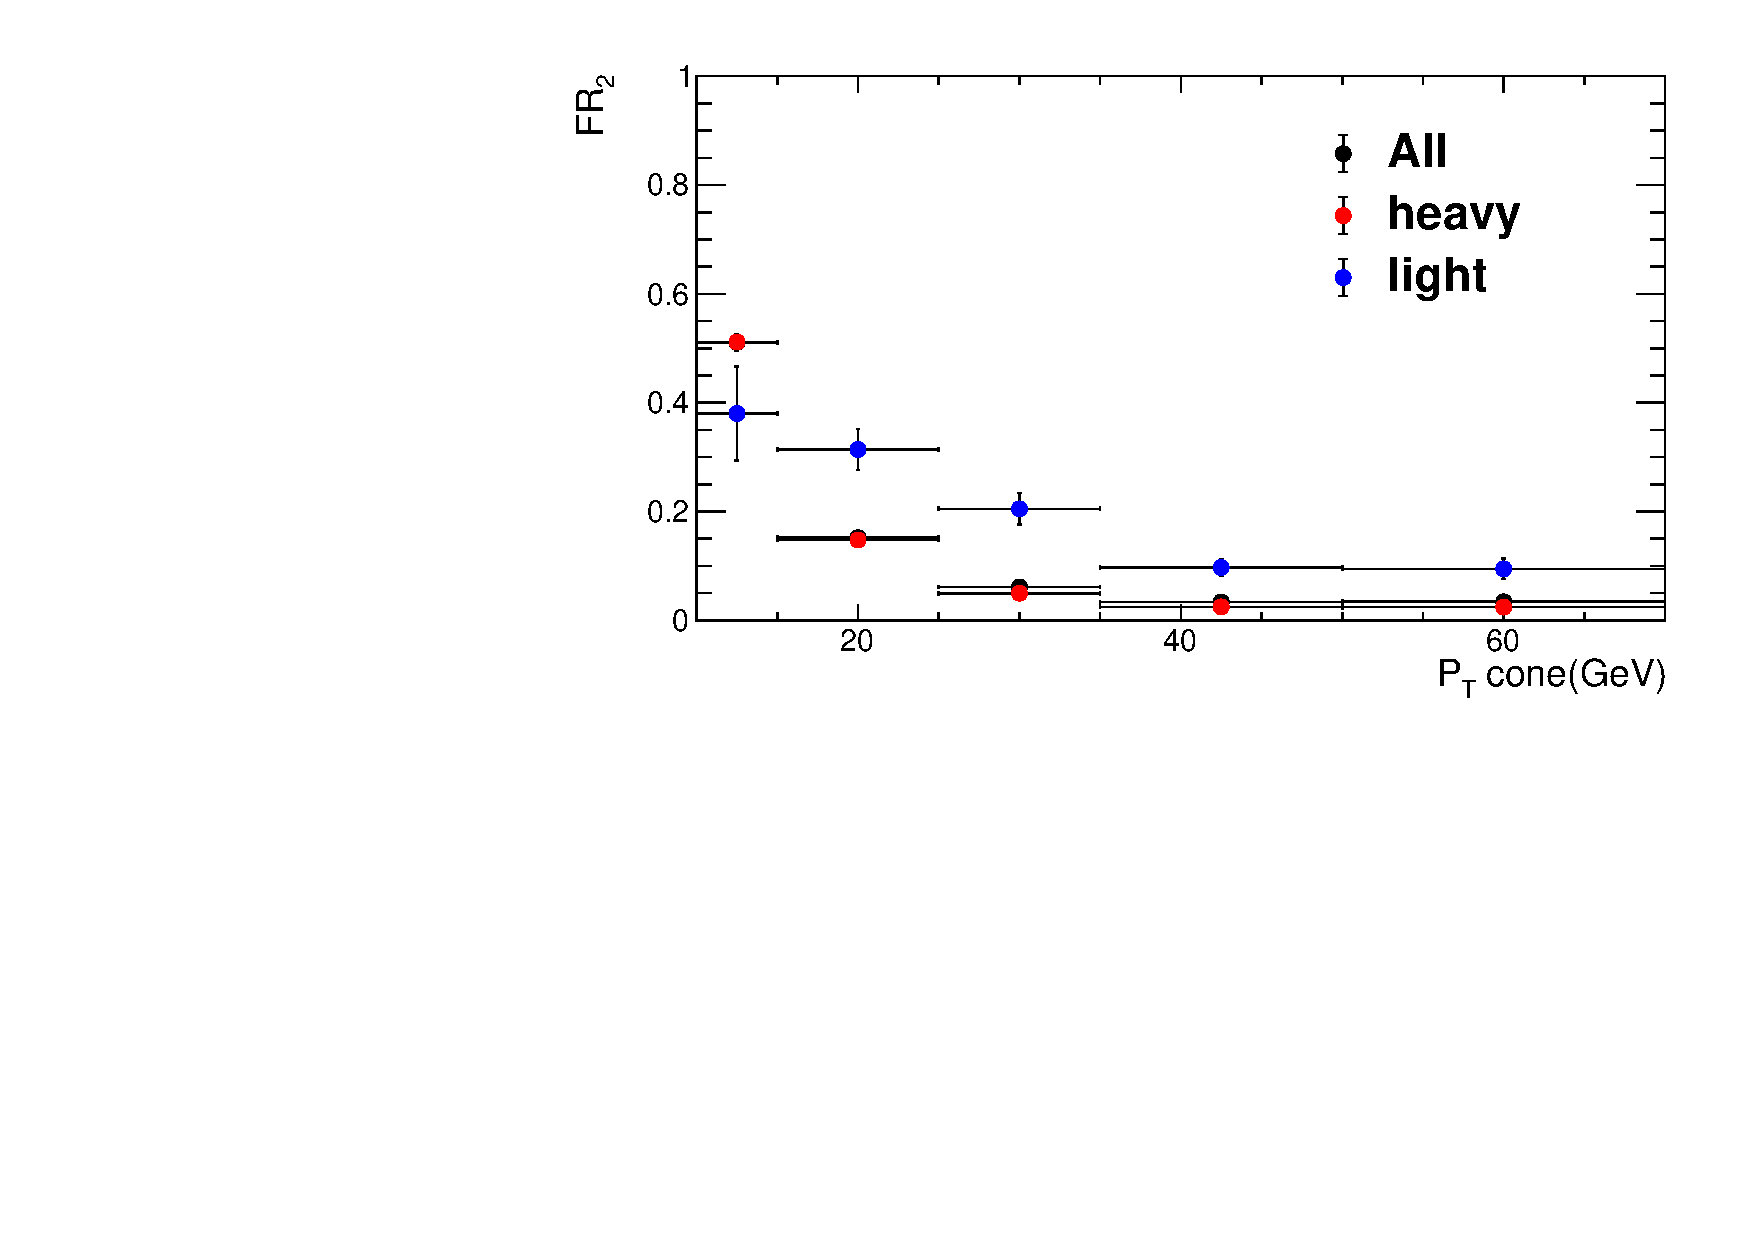
\includegraphics[width=.48\textwidth]{Figures/c6/backgrounds/FR/sFR/QCD/LeptonPt_ele_eta2_FR2.pdf}
  \hfill{}
  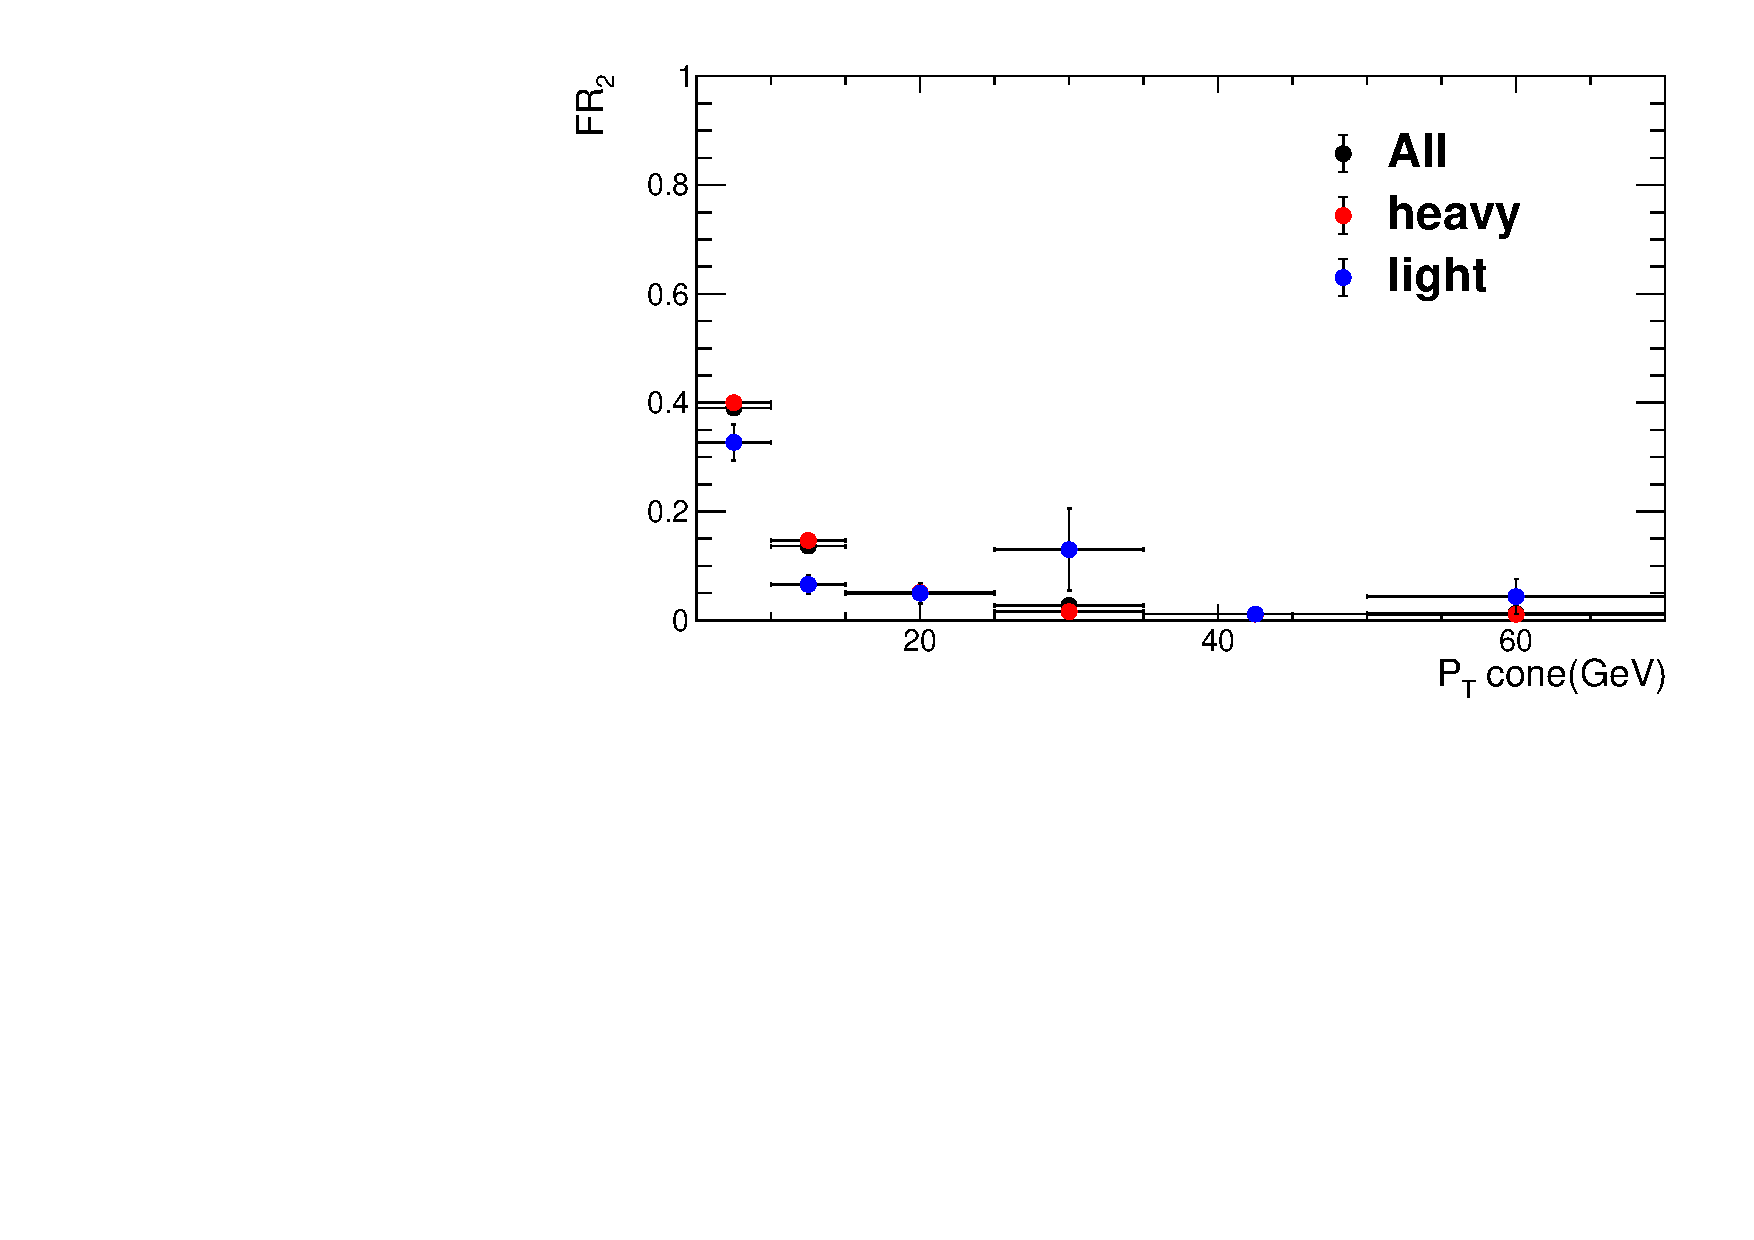
\includegraphics[width=.48\textwidth]{Figures/c6/backgrounds/FR/sFR/QCD/LeptonPt_mu_eta2_FR2.pdf}\\
  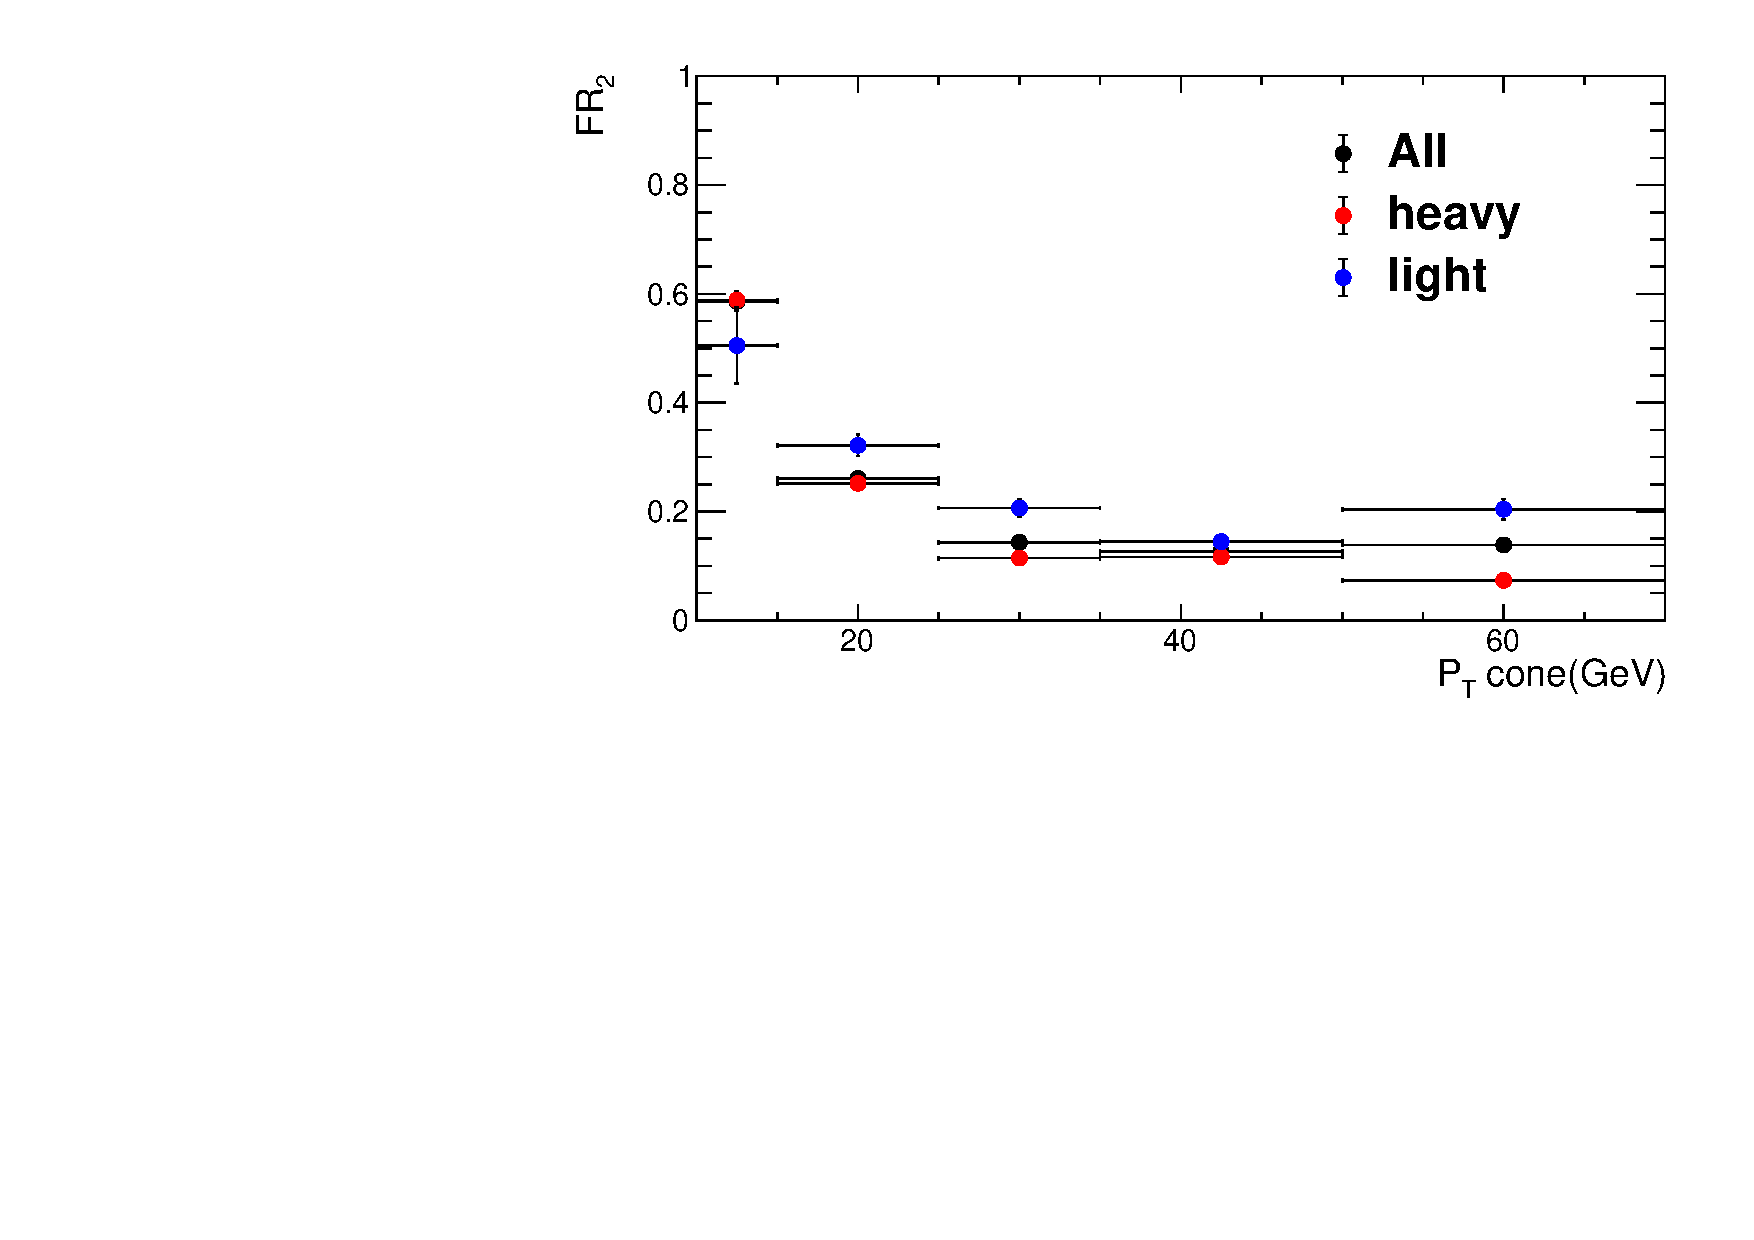
\includegraphics[width=.48\textwidth]{Figures/c6/backgrounds/FR/sFR/QCD/LeptonPt_ele_eta3_FR2.pdf}
  \hfill{}
  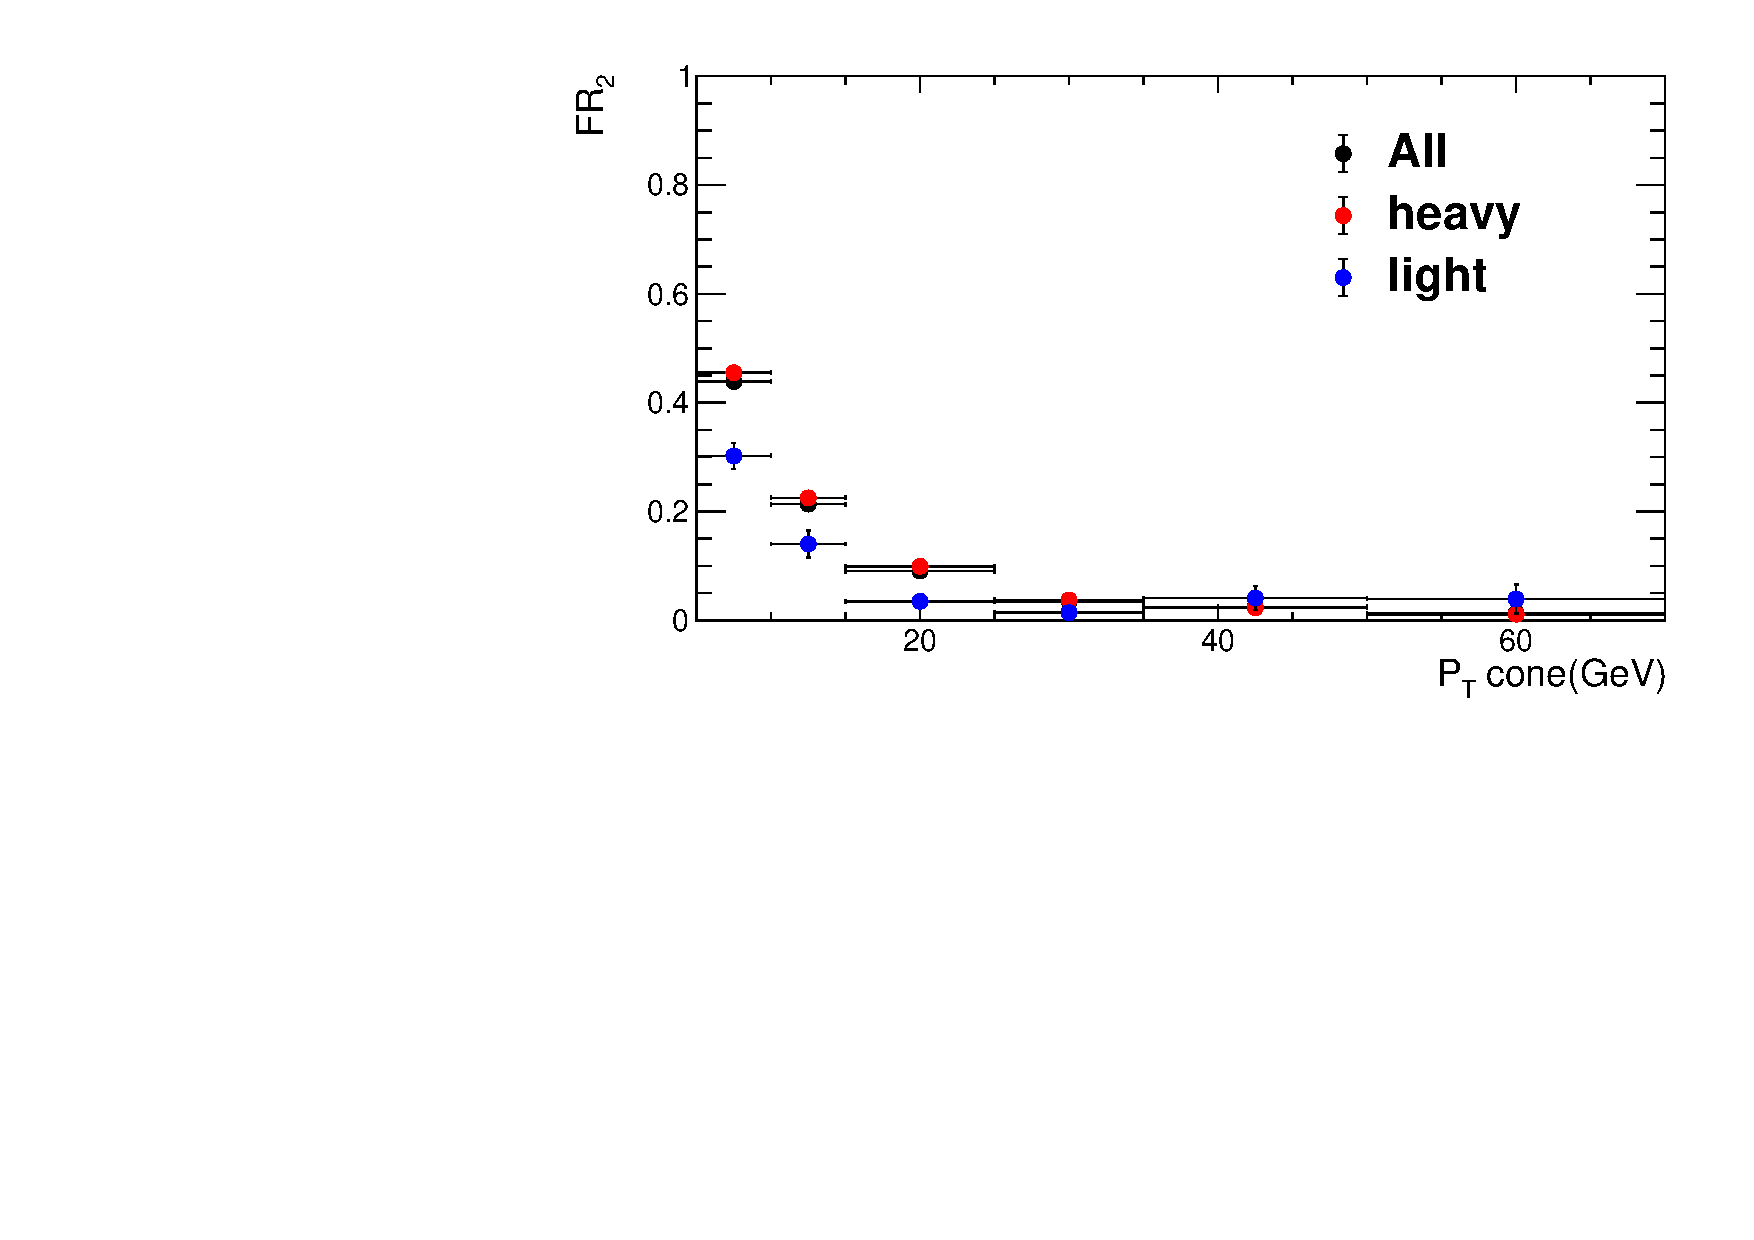
\includegraphics[width=.48\textwidth]{Figures/c6/backgrounds/FR/sFR/QCD/LeptonPt_mu_eta3_FR2.pdf}\\
  \caption{Single fake rates obtained in 2016 simulation for electrons
    (left) and muons (right) as a function of \ptc, for \abseta ranges
    $[0,0.8]$ (top), $[0.8,1.479]$ (middle), and $[1.479,2.5]$
    (bottom). The different histograms represent the contributions
    from light- and heavy-quark hadrons, and their average.}
  \label{fig:sFR_mc}
\end{figure}

\begin{figure}[t!]
  \centering
  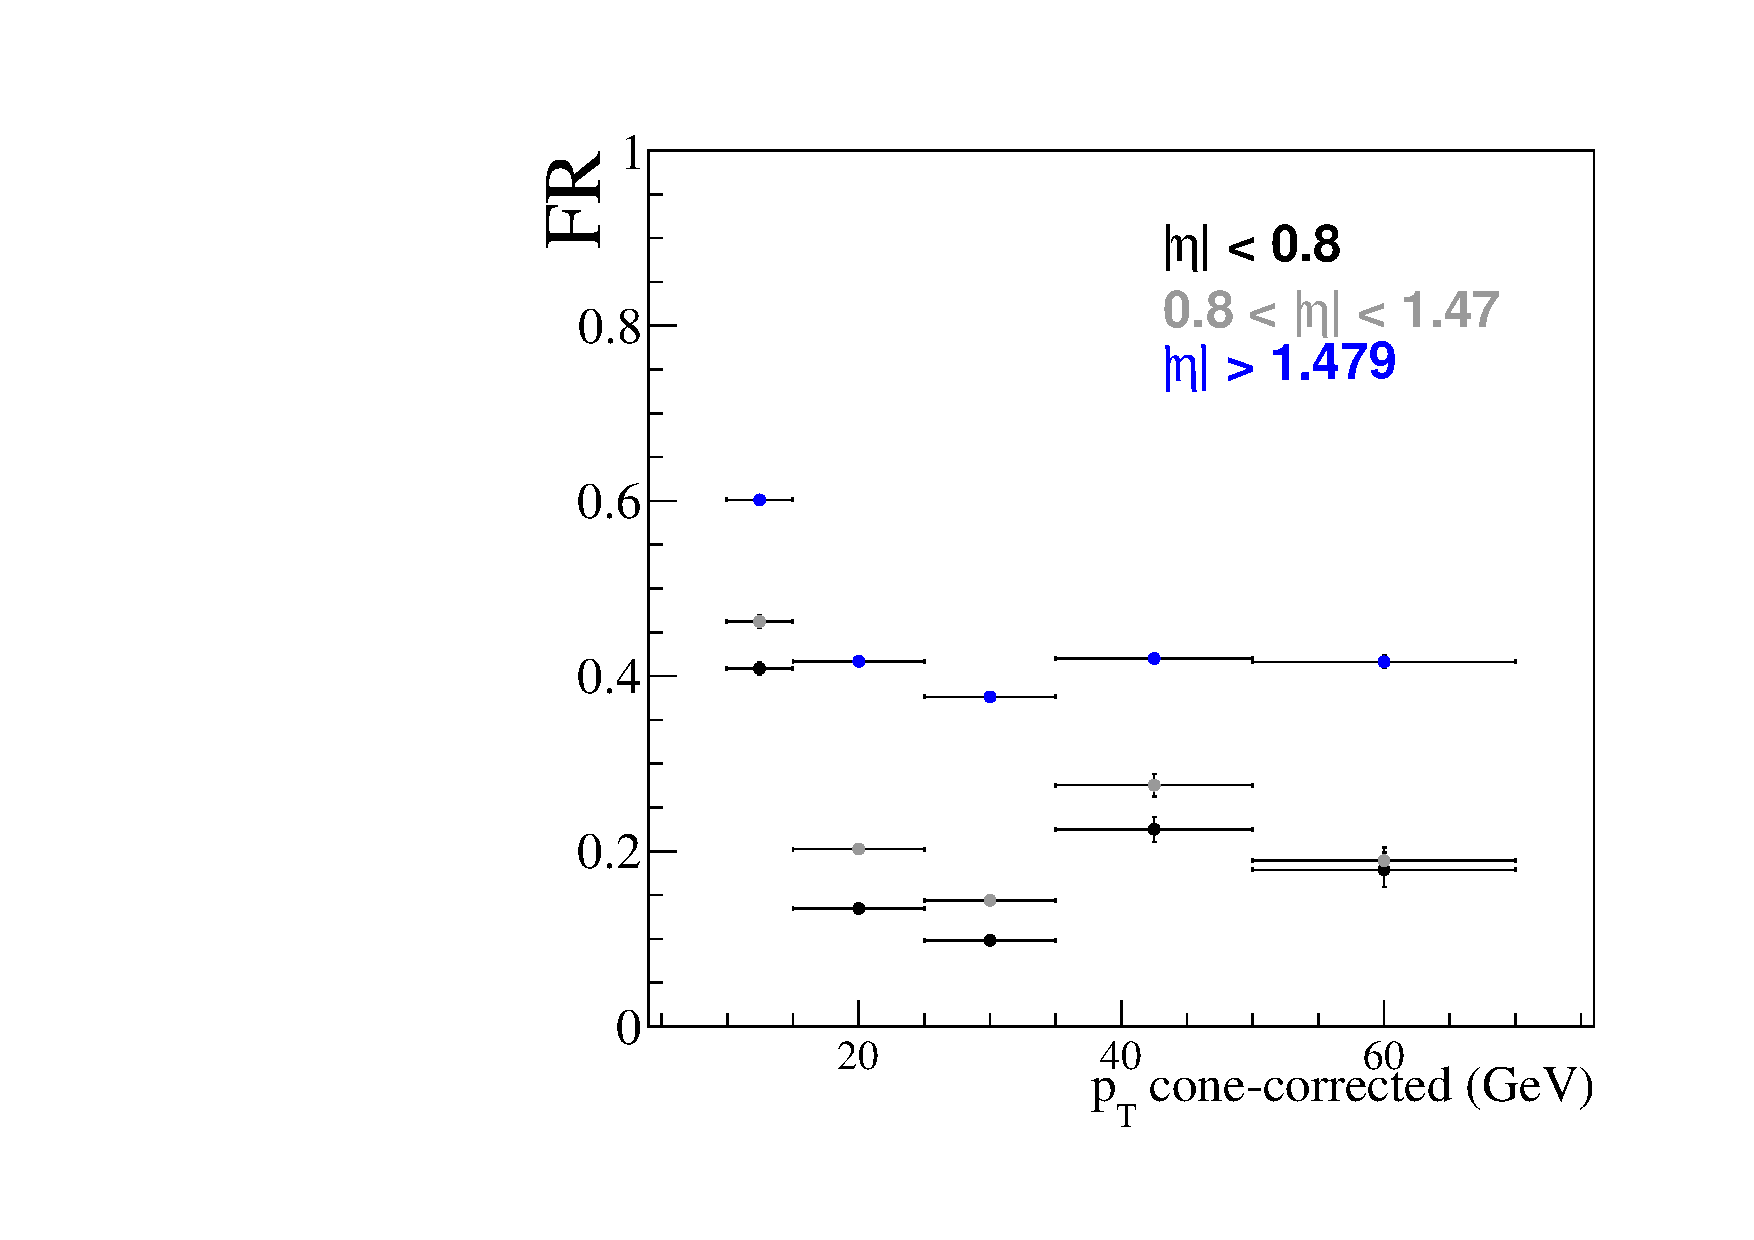
\includegraphics[width=.46\textwidth]{Figures/c6/backgrounds/FR/sFR/data/electrons.pdf}
  \hfill{}
  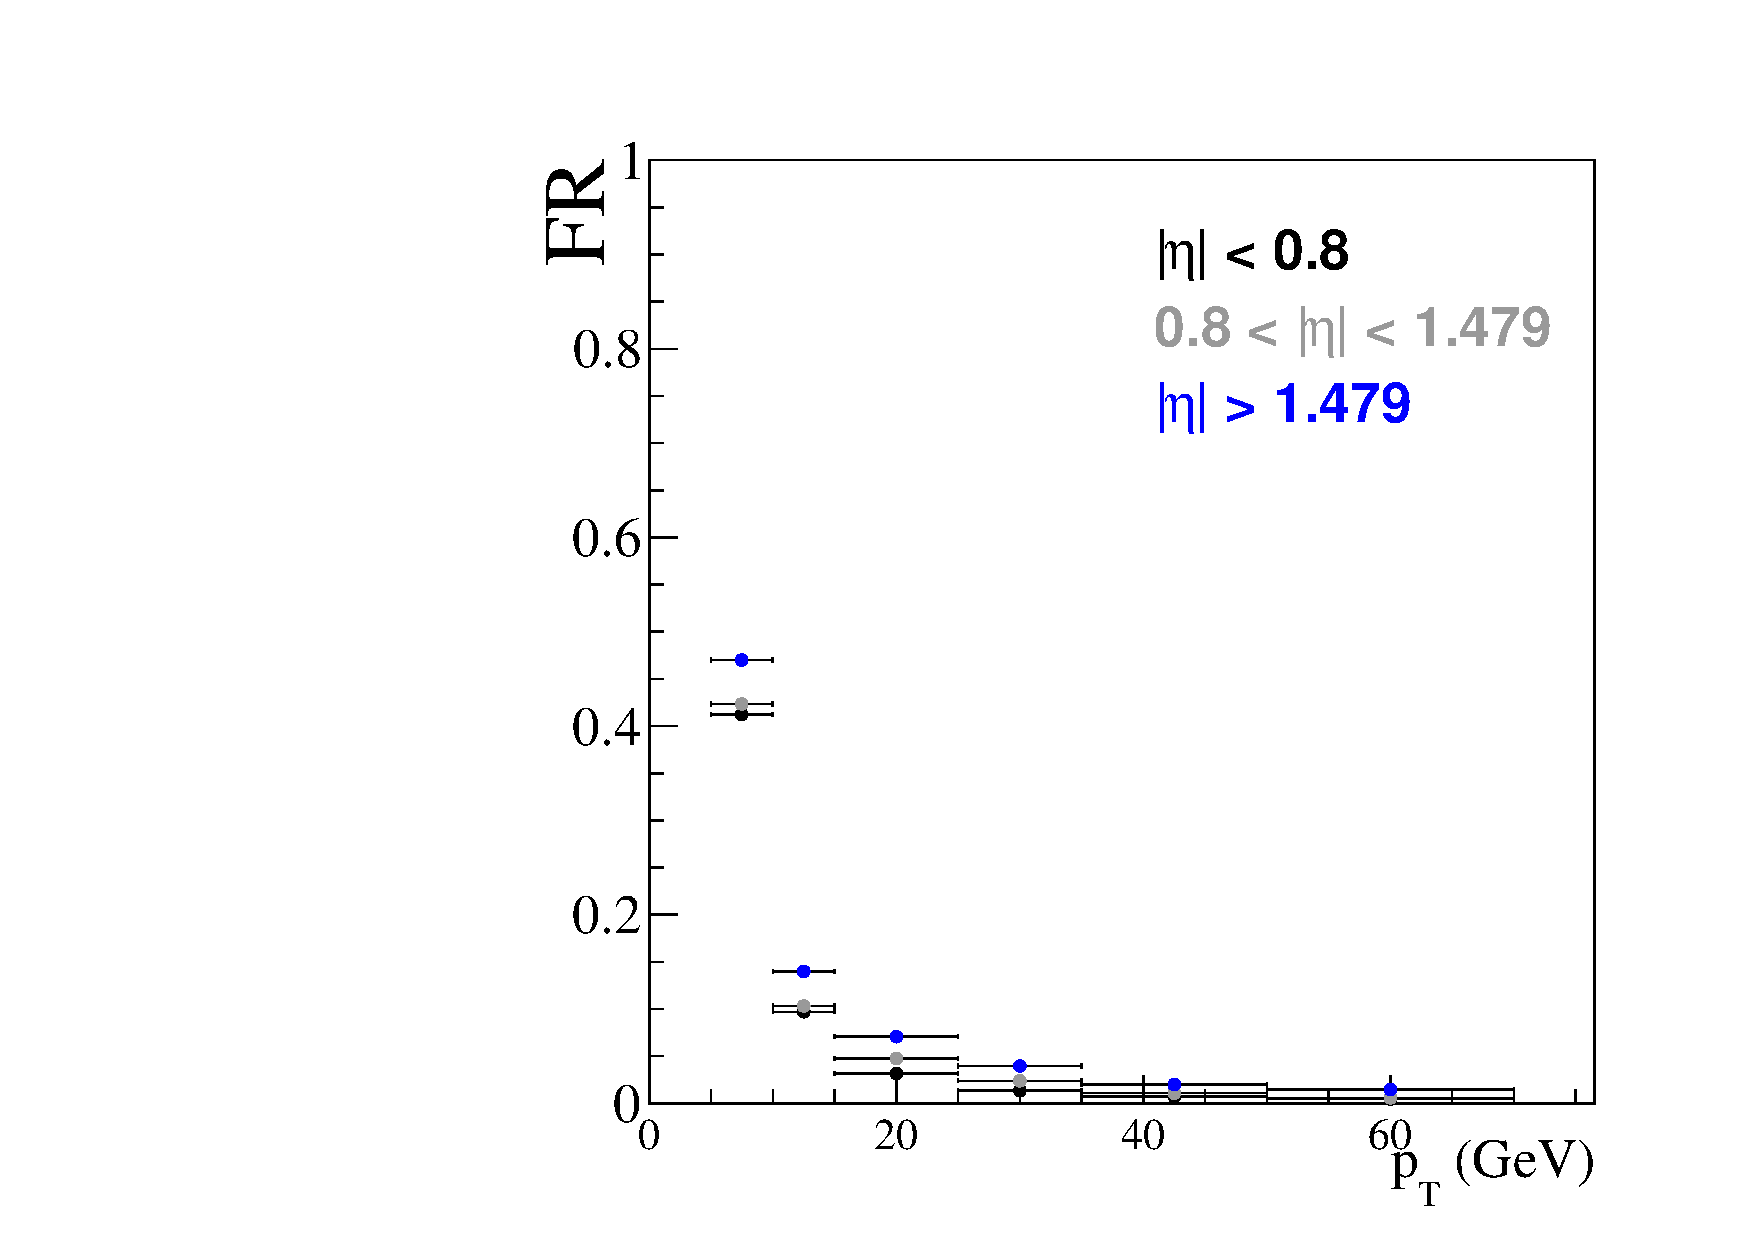
\includegraphics[height=6.4cm, width=7.0cm]{Figures/c6/backgrounds/FR/sFR/data/muons.pdf}\\
  \caption{Single fake rates measured in 2016 data for electrons (left) and
    muons (right) as a function of \ptc, for \abseta ranges $[0,0.8]$
    (top), $[0.8,1.479]$ (middle), and $[1.479,2.5]$ (bottom).}
  \label{fig:sFR_data}
\end{figure}

%% Figures~\ref{fig:sFR_comp_ele} and \ref{fig:sFR_comp_muo} show in
%% simulation that the contributions to \sfr from light-quark and
%% heavy-quark hadrons are comparable, which is a necessary requirement
%% in order to apply \sfr independently of the flavor composition in the
%% application region.
%% \begin{figure}[t!]
%%   \centering
%%   \includegraphics[width=.32\textwidth]{figs/placeholder.png}
%%   \hfill{}
%%   \includegraphics[width=.32\textwidth]{figs/placeholder.png}
%%   \hfill{}
%%   \includegraphics[width=.32\textwidth]{figs/placeholder.png}
%%   \caption{Single fake-electron rates computed in simulation as a
%%     function of \ptc, for \abseta ranges $[0,0.8]$ (left),
%%     $[0.8,1.479]$ (center), and $[1.479,2.5]$ (right), separately for
%%     electrons from light-quark and heavy-quark hadron decays.}
%%   \label{fig:sFR_comp_ele}
%% \end{figure}
%% \begin{figure}[t!]
%%   \centering
%%   \includegraphics[width=.32\textwidth]{figs/placeholder.png}
%%   \hfill{}
%%   \includegraphics[width=.32\textwidth]{figs/placeholder.png}
%%   \hfill{}
%%   \includegraphics[width=.32\textwidth]{figs/placeholder.png}
%%   \caption{Single fake-muon rates computed in simulation as a
%%     function of \ptc, for \abseta ranges $[0,0.8]$ (left),
%%     $[0.8,1.479]$ (center), and $[1.479,2.4]$ (right), separately for
%%     muons from light-quark and heavy-quark hadron decays.}
%%   \label{fig:sFR_comp_muo}
%% \end{figure}

Figures~\ref{fig:sFR_dxy} and ~\ref{fig:sFR_dxy_comparison} show that \sfr values are fairly independent
of the lepton \dxy.
\begin{figure}[t!]
  \centering
  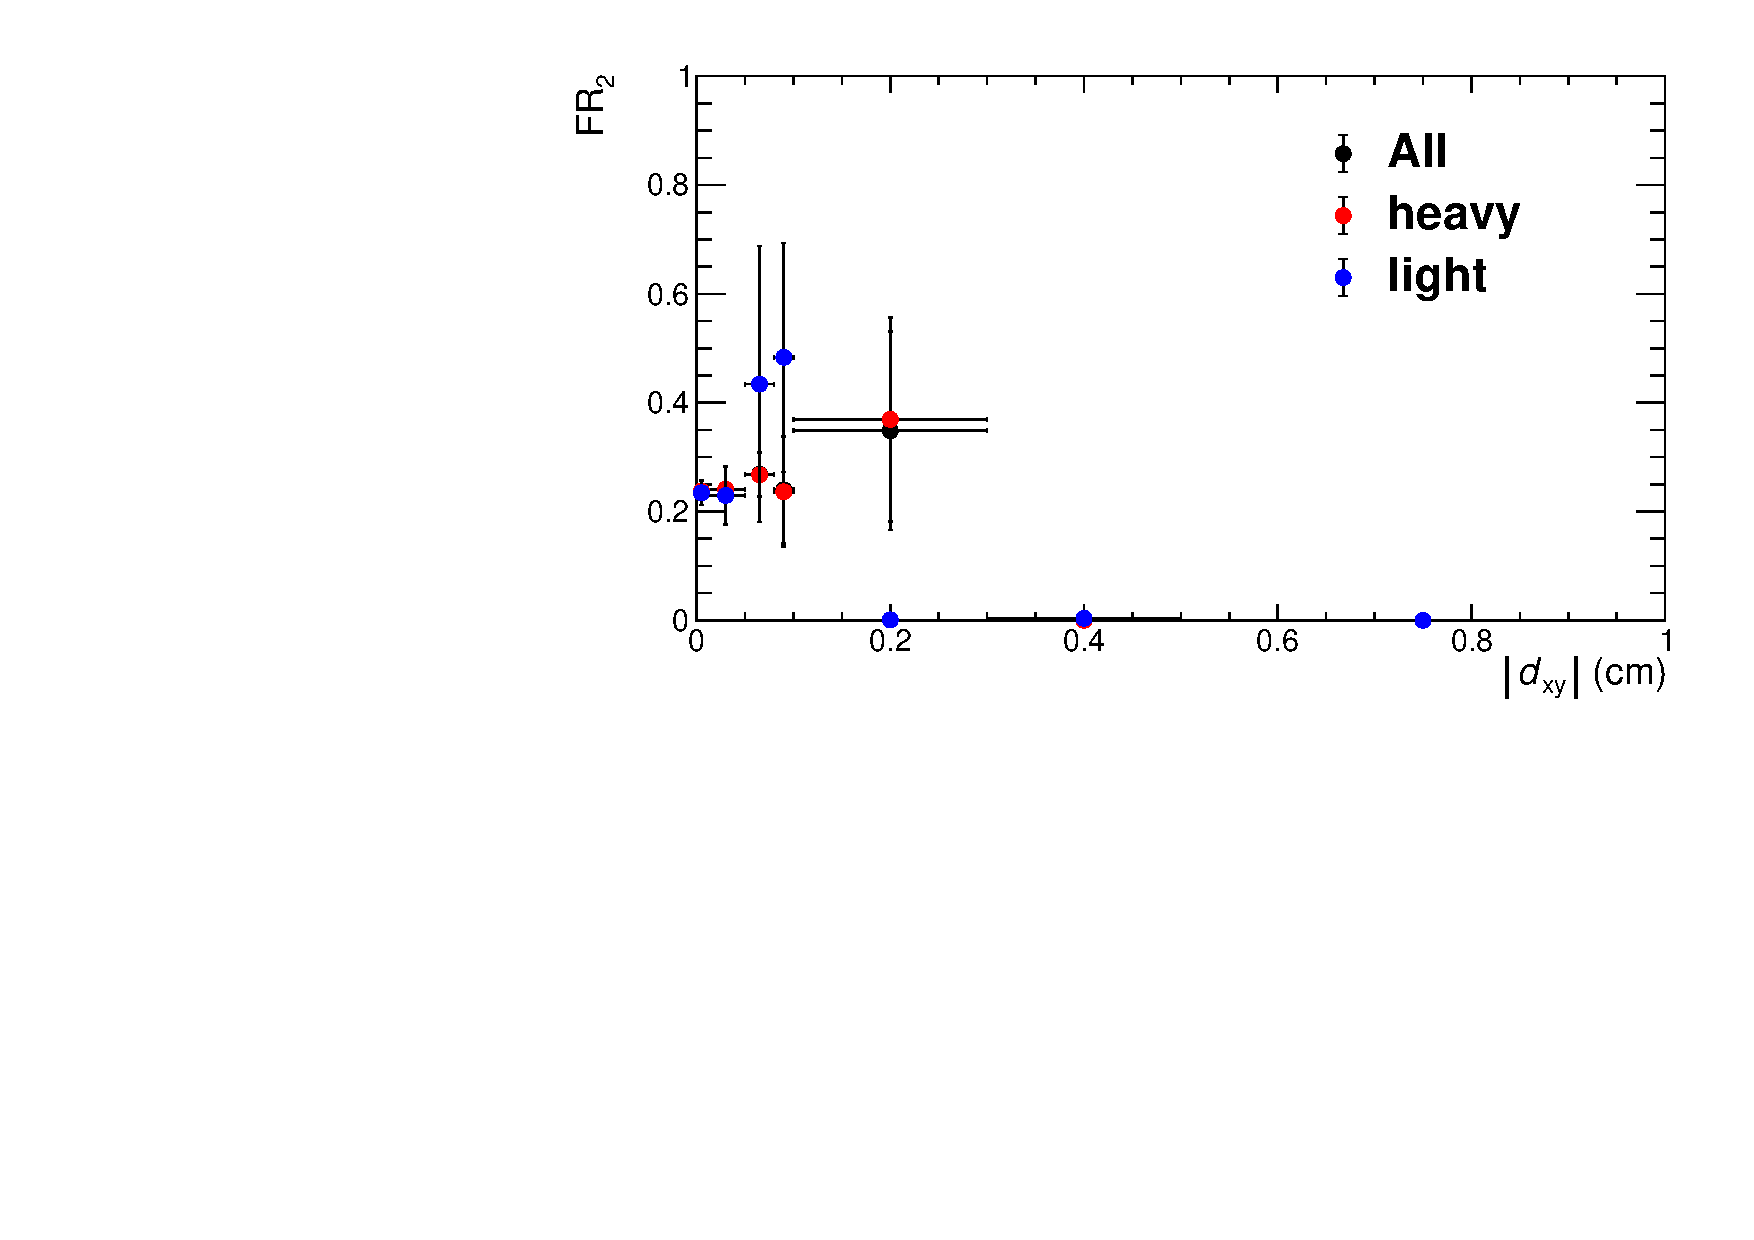
\includegraphics[width=.48\textwidth]{Figures/c6/backgrounds/FR/sFR/QCD/dxy_ele_eta1_FR2.pdf}
  \hfill{}
  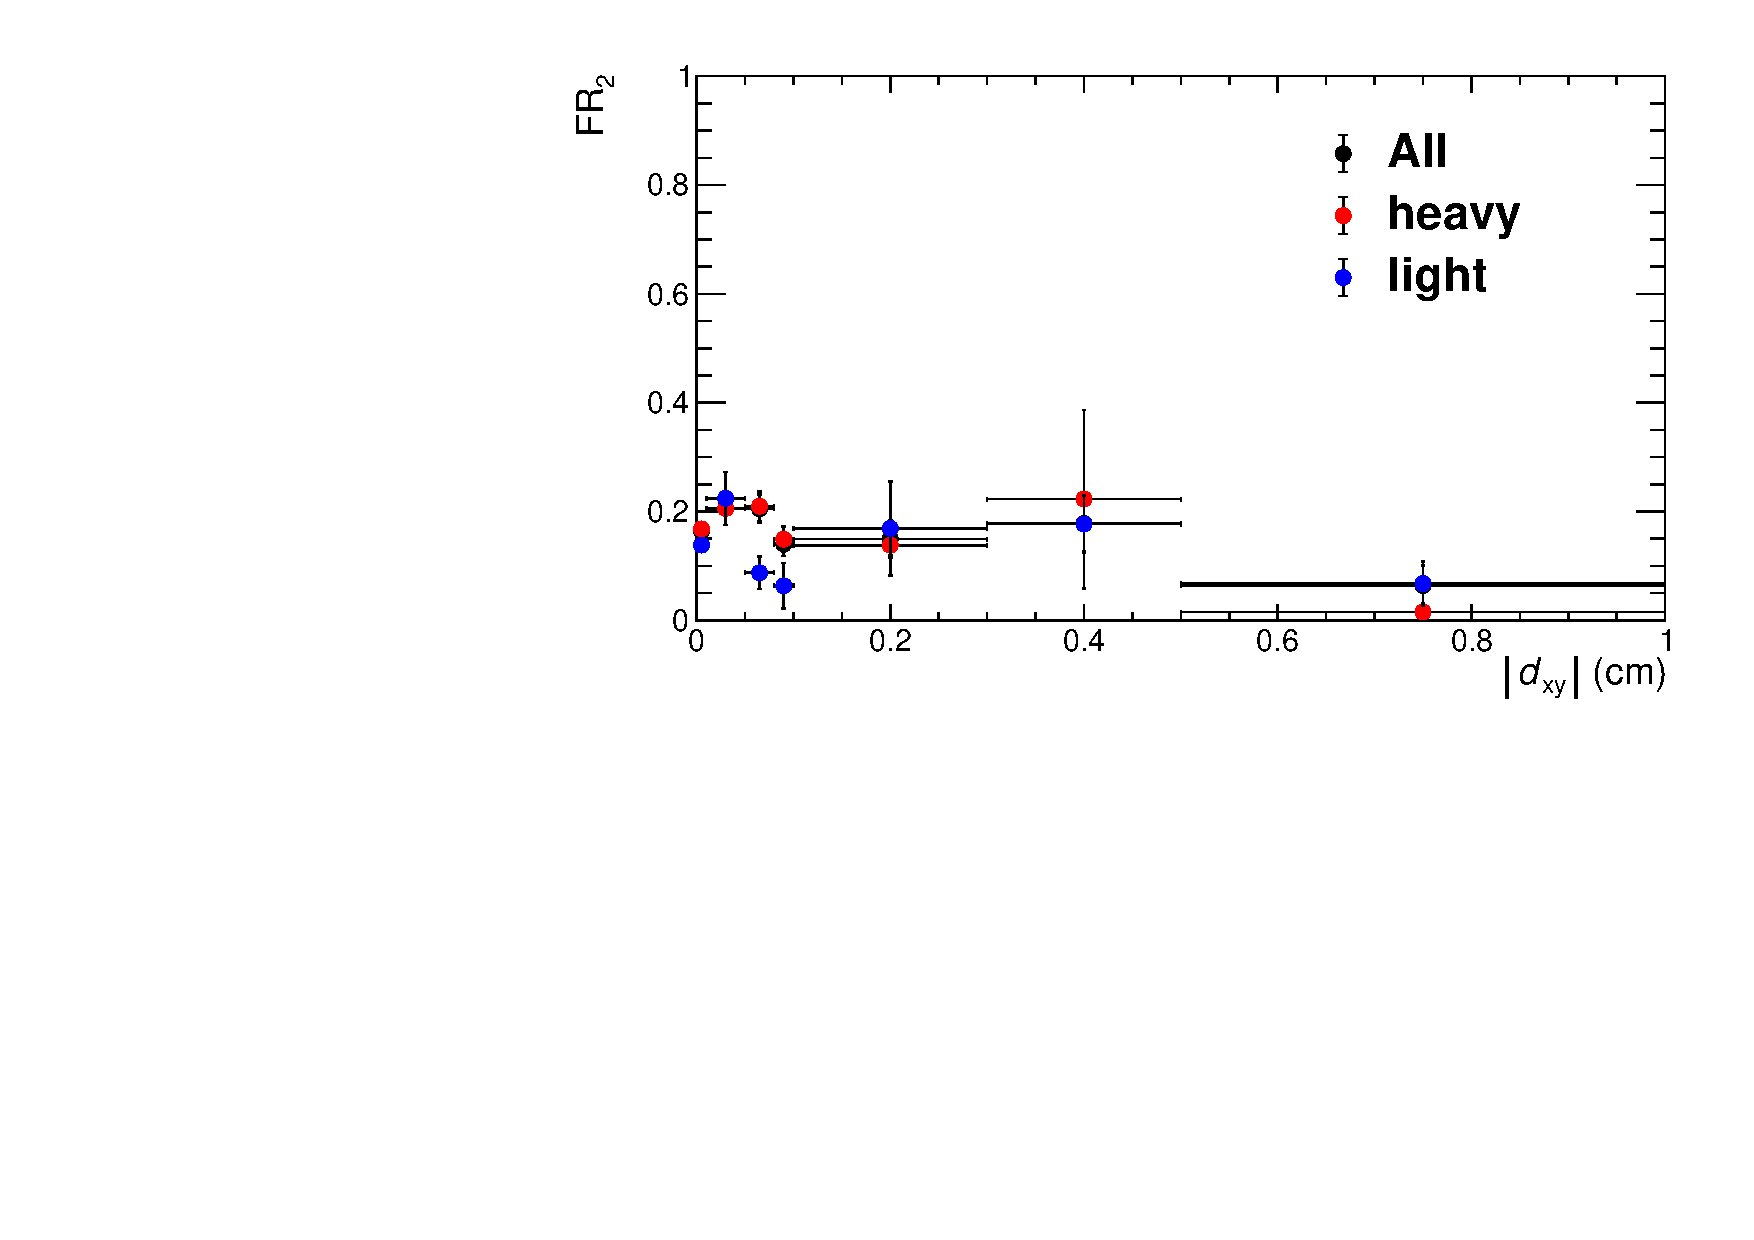
\includegraphics[width=.48\textwidth]{Figures/c6/backgrounds/FR/sFR/QCD/dxy_mu_eta1_FR2.pdf}\\
  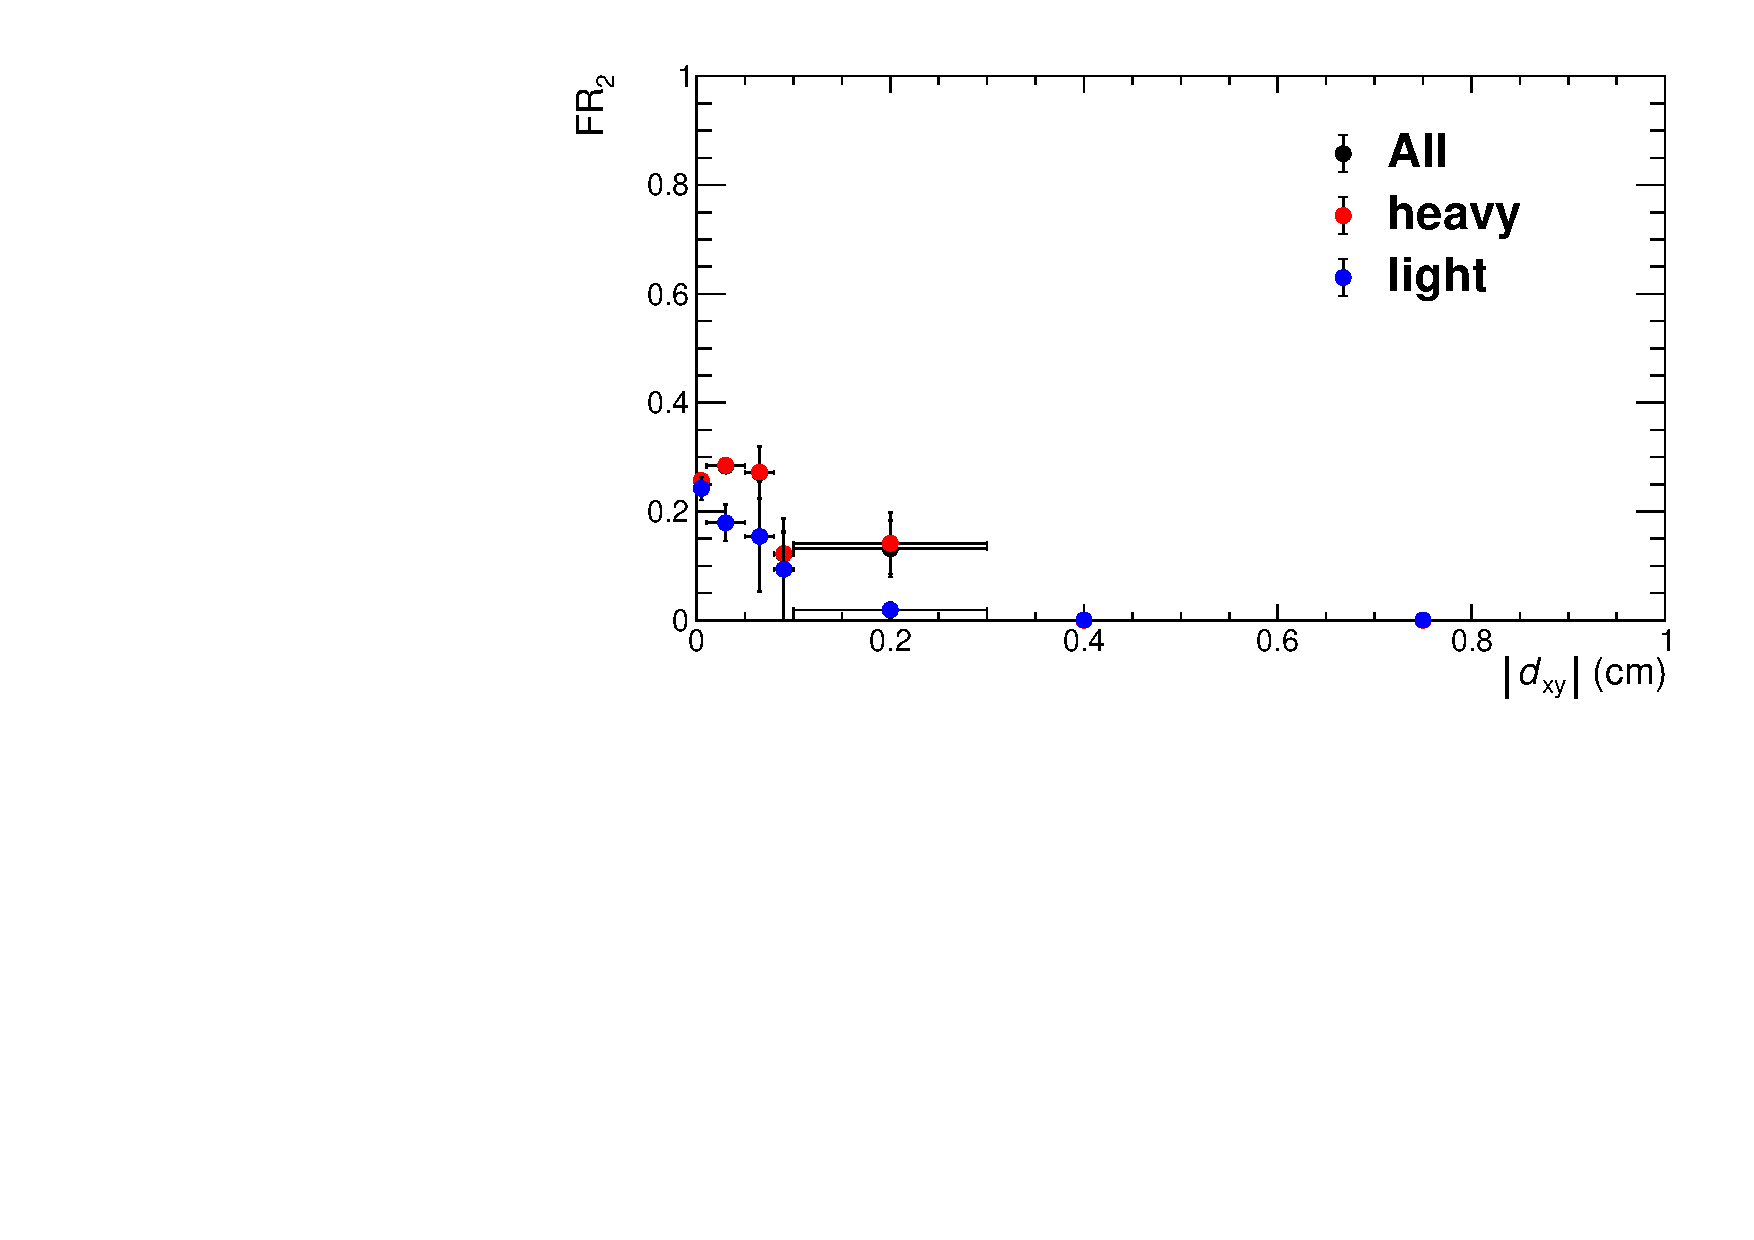
\includegraphics[width=.48\textwidth]{Figures/c6/backgrounds/FR/sFR/QCD/dxy_ele_eta2_FR2.pdf}
  \hfill{}
  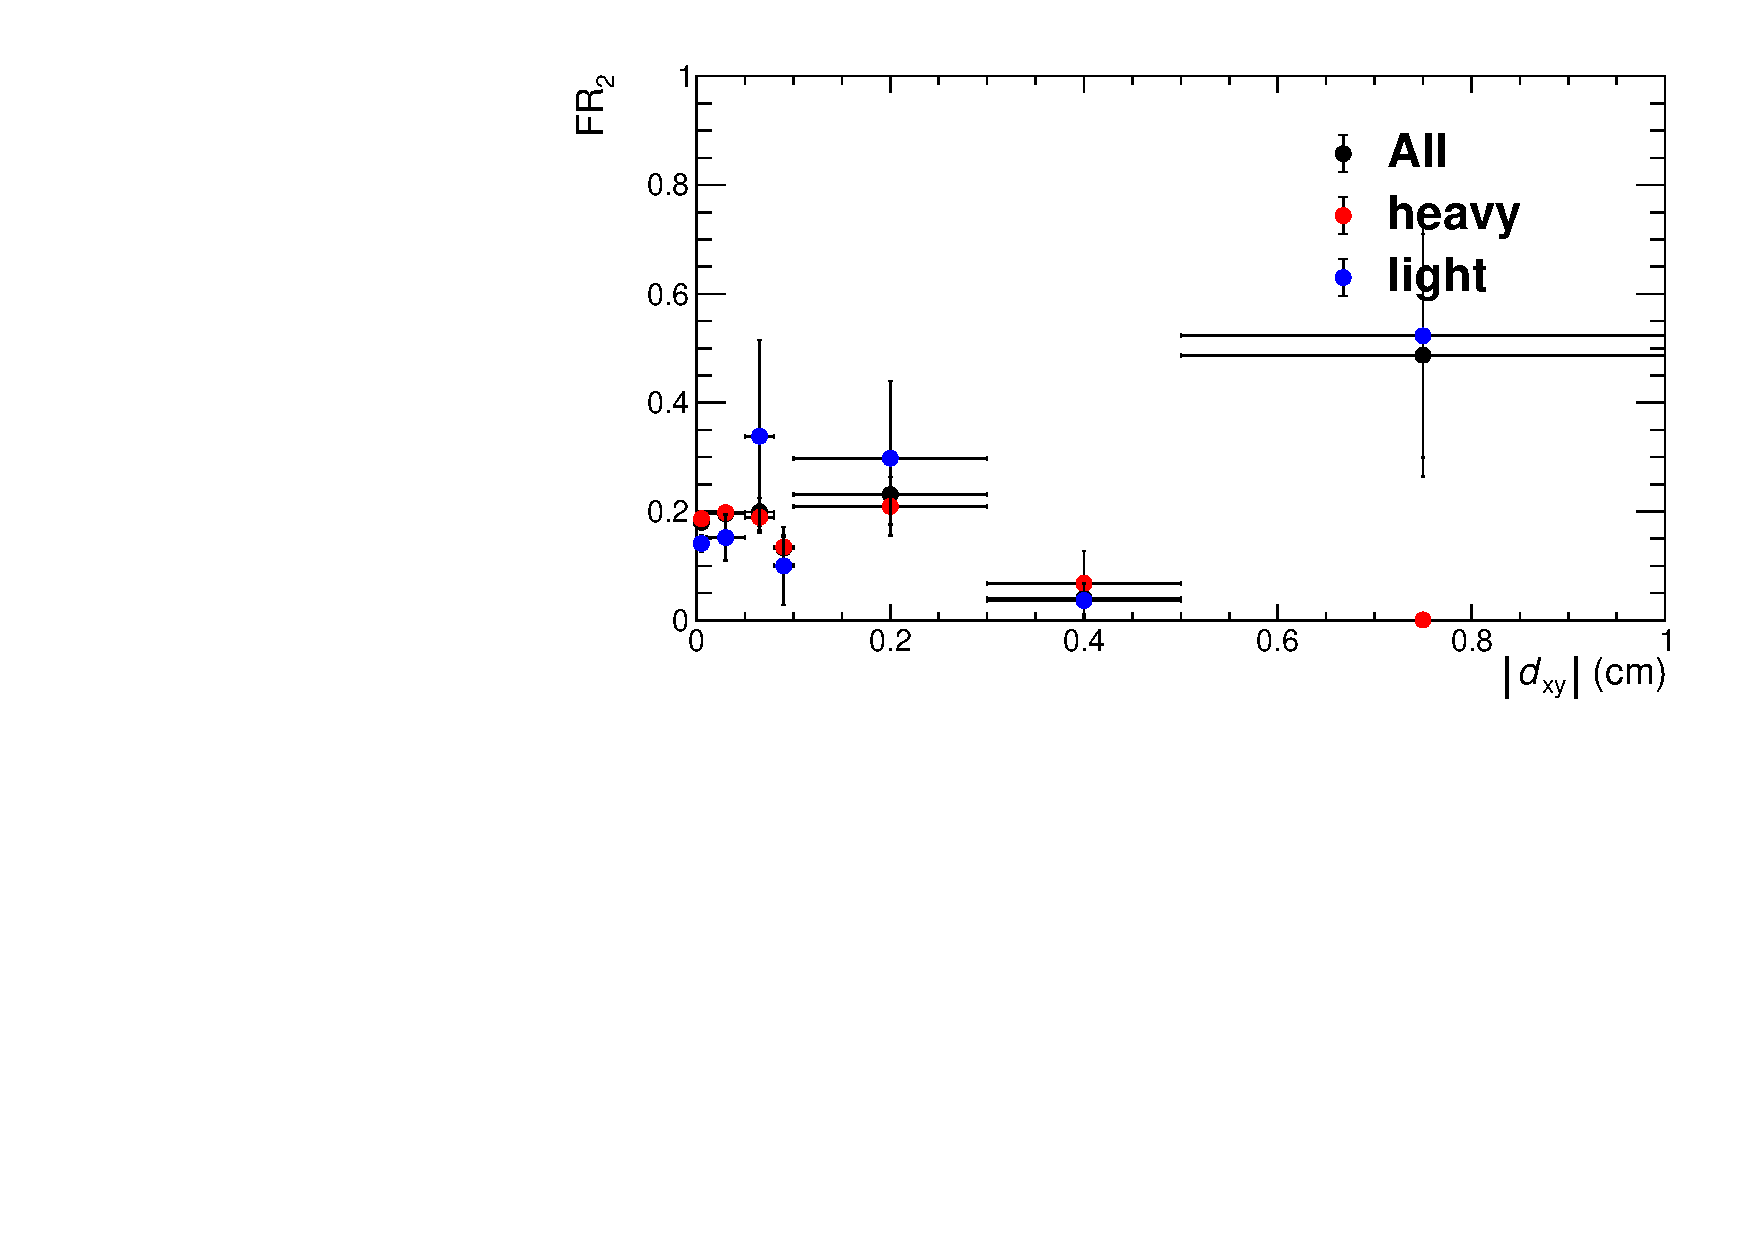
\includegraphics[width=.48\textwidth]{Figures/c6/backgrounds/FR/sFR/QCD/dxy_mu_eta2_FR2.pdf}\\
  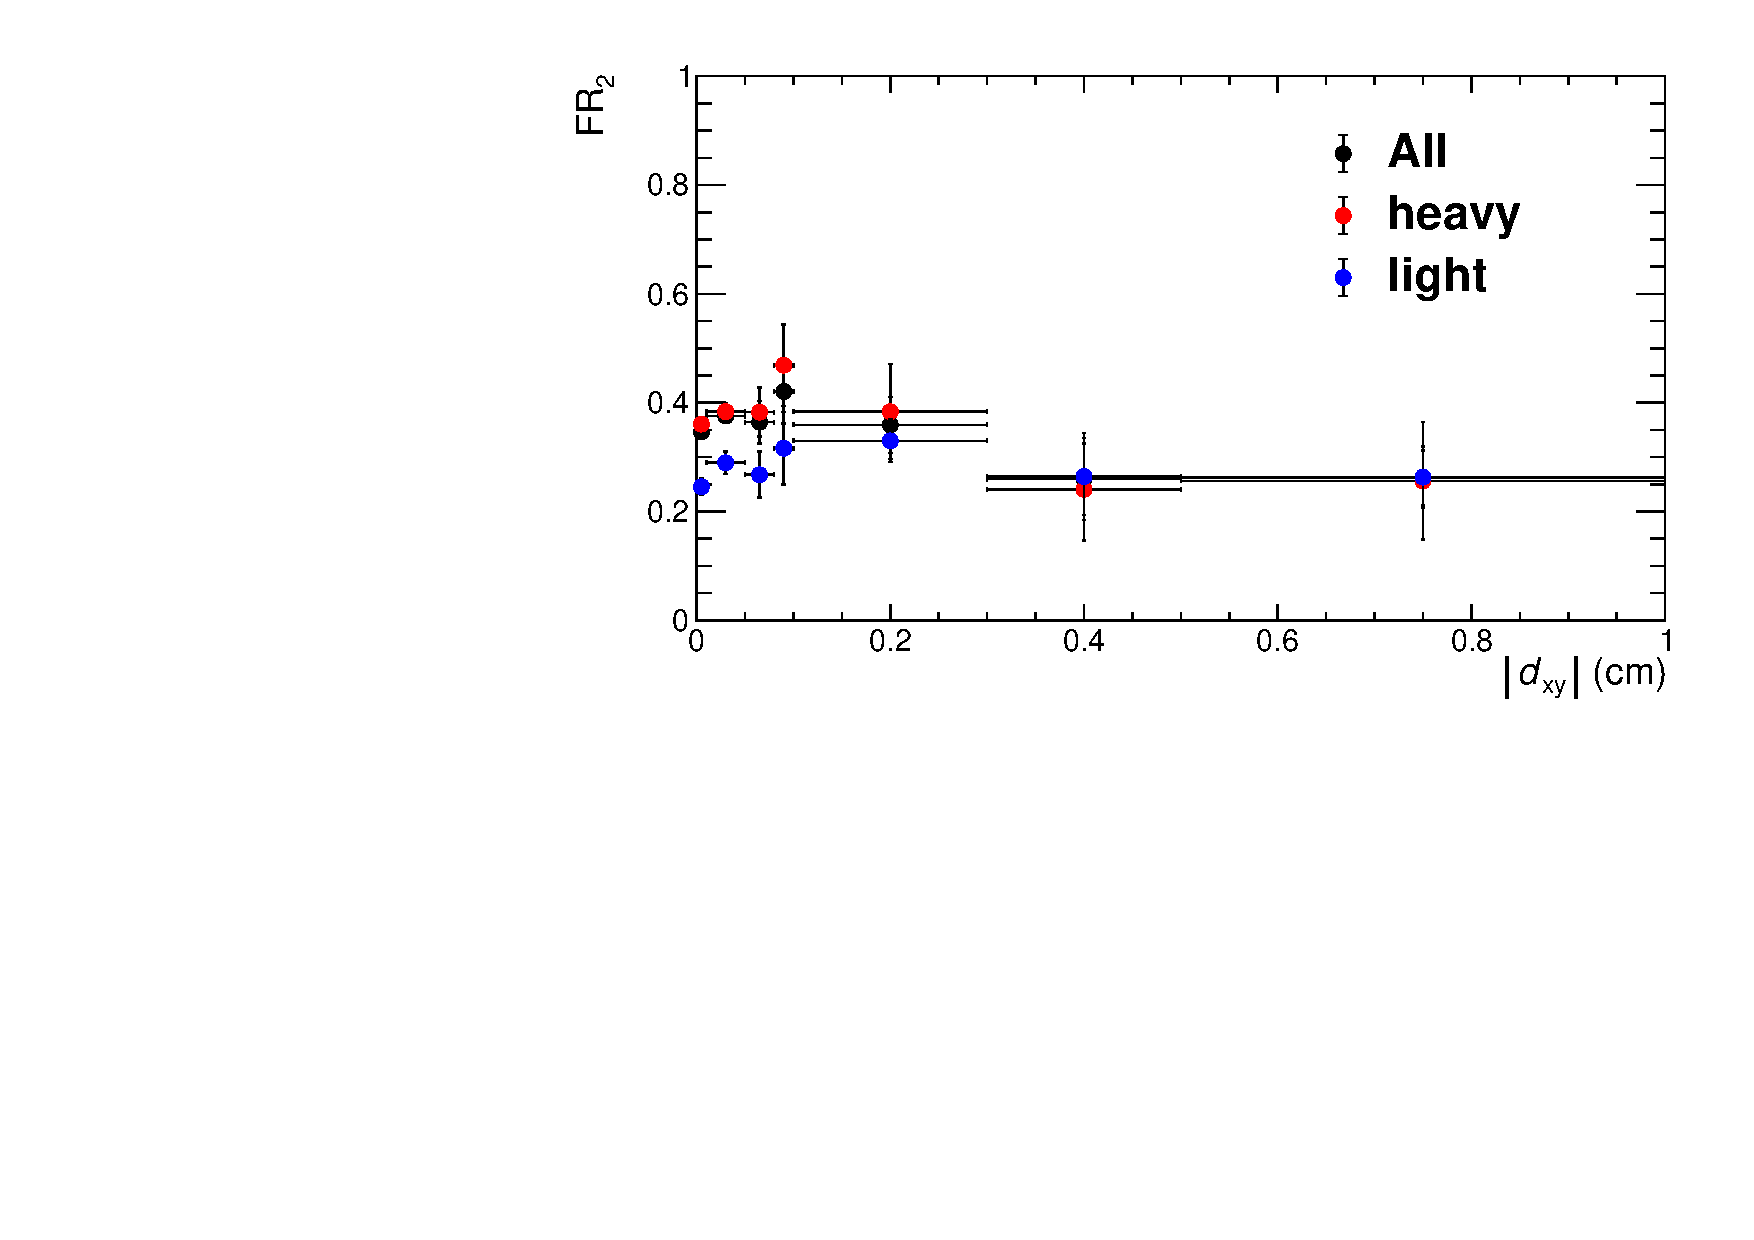
\includegraphics[width=.48\textwidth]{Figures/c6/backgrounds/FR/sFR/QCD/dxy_ele_eta3_FR2.pdf}
  \hfill{}
  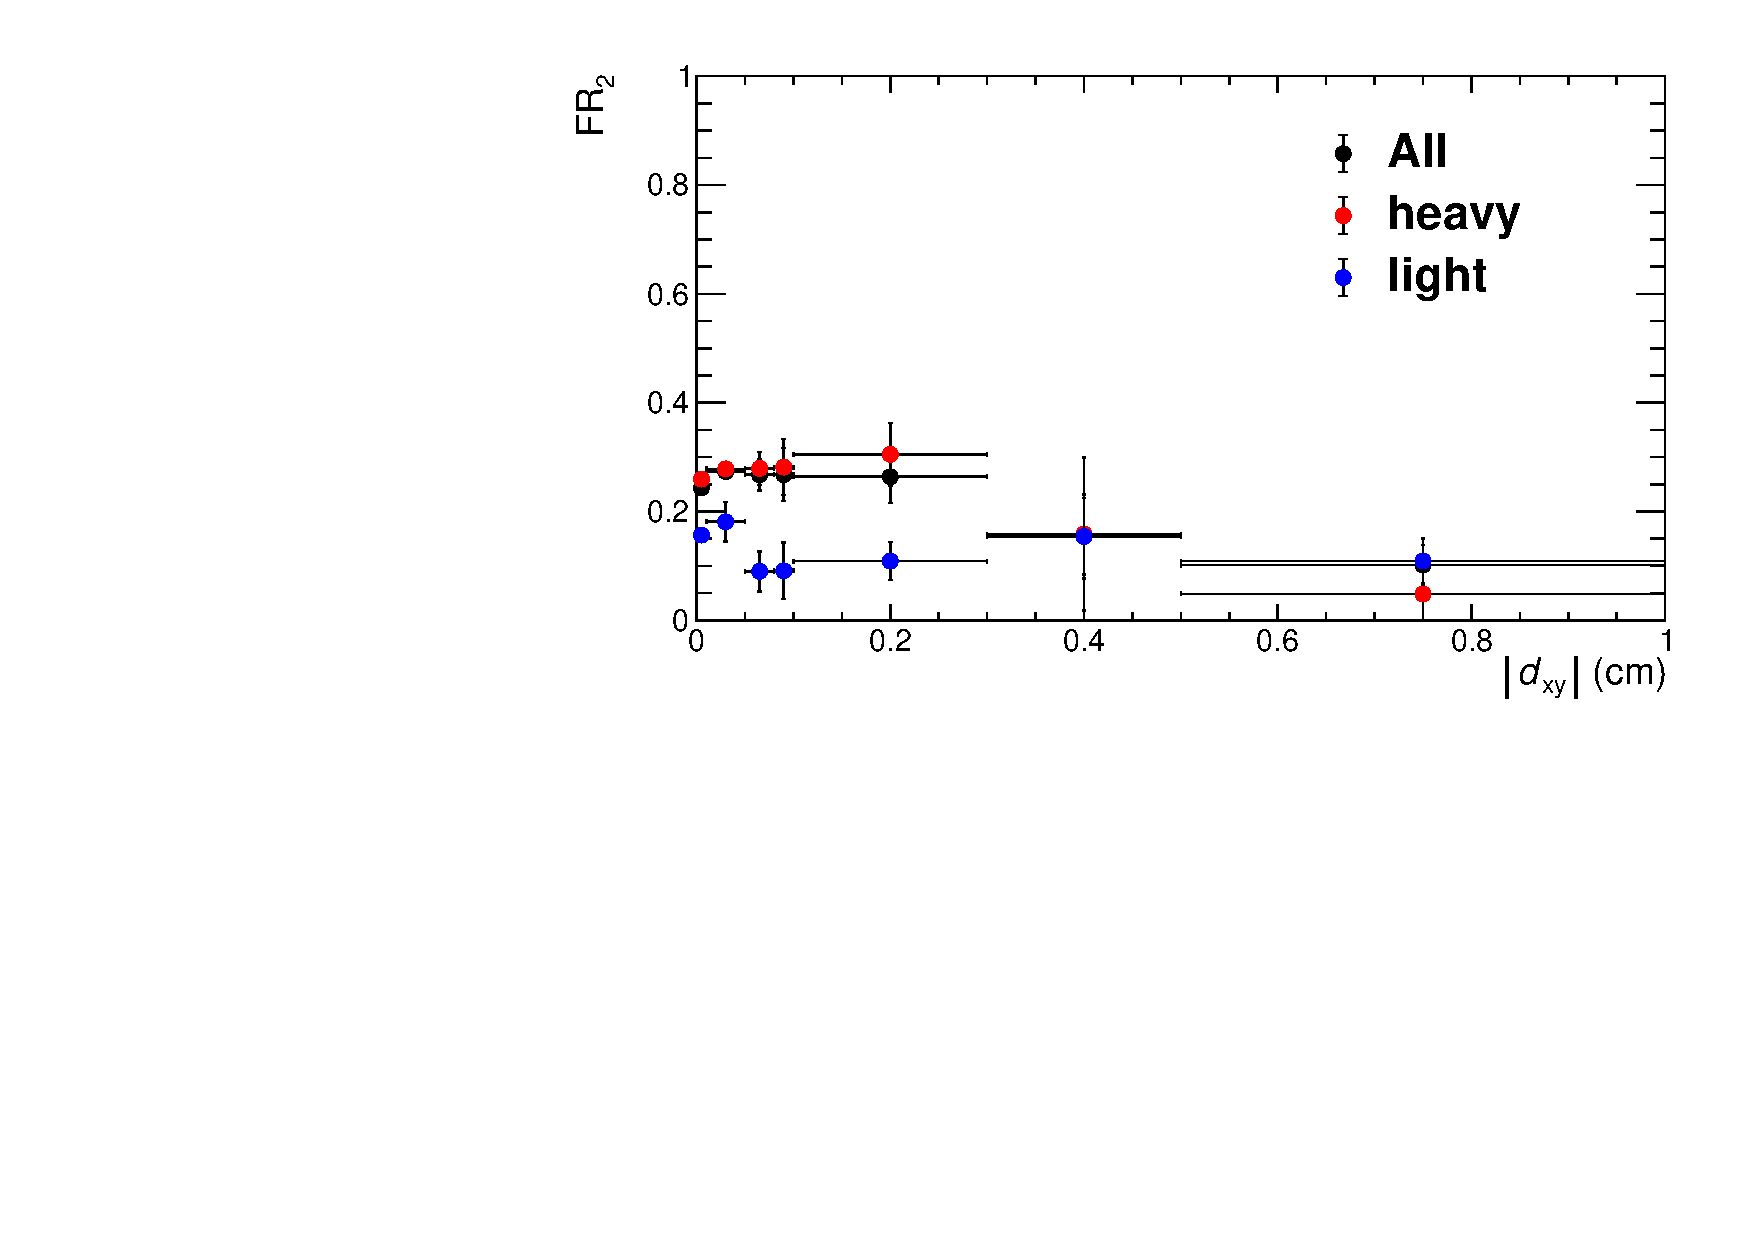
\includegraphics[width=.48\textwidth]{Figures/c6/backgrounds/FR/sFR/QCD/dxy_mu_eta3_FR2.pdf}
  \caption{Single fake rates obtained in 2016 simulation for electrons
    (left) and muons (right) as
    a function of \dxy, for \abseta ranges $[0,0.8]$ (top),
    $[0.8,1.479]$ (middle), and $[1.479,2.5]$ (bottom).}
  \label{fig:sFR_dxy}
\end{figure}

\begin{figure}[t!]
  \centering
  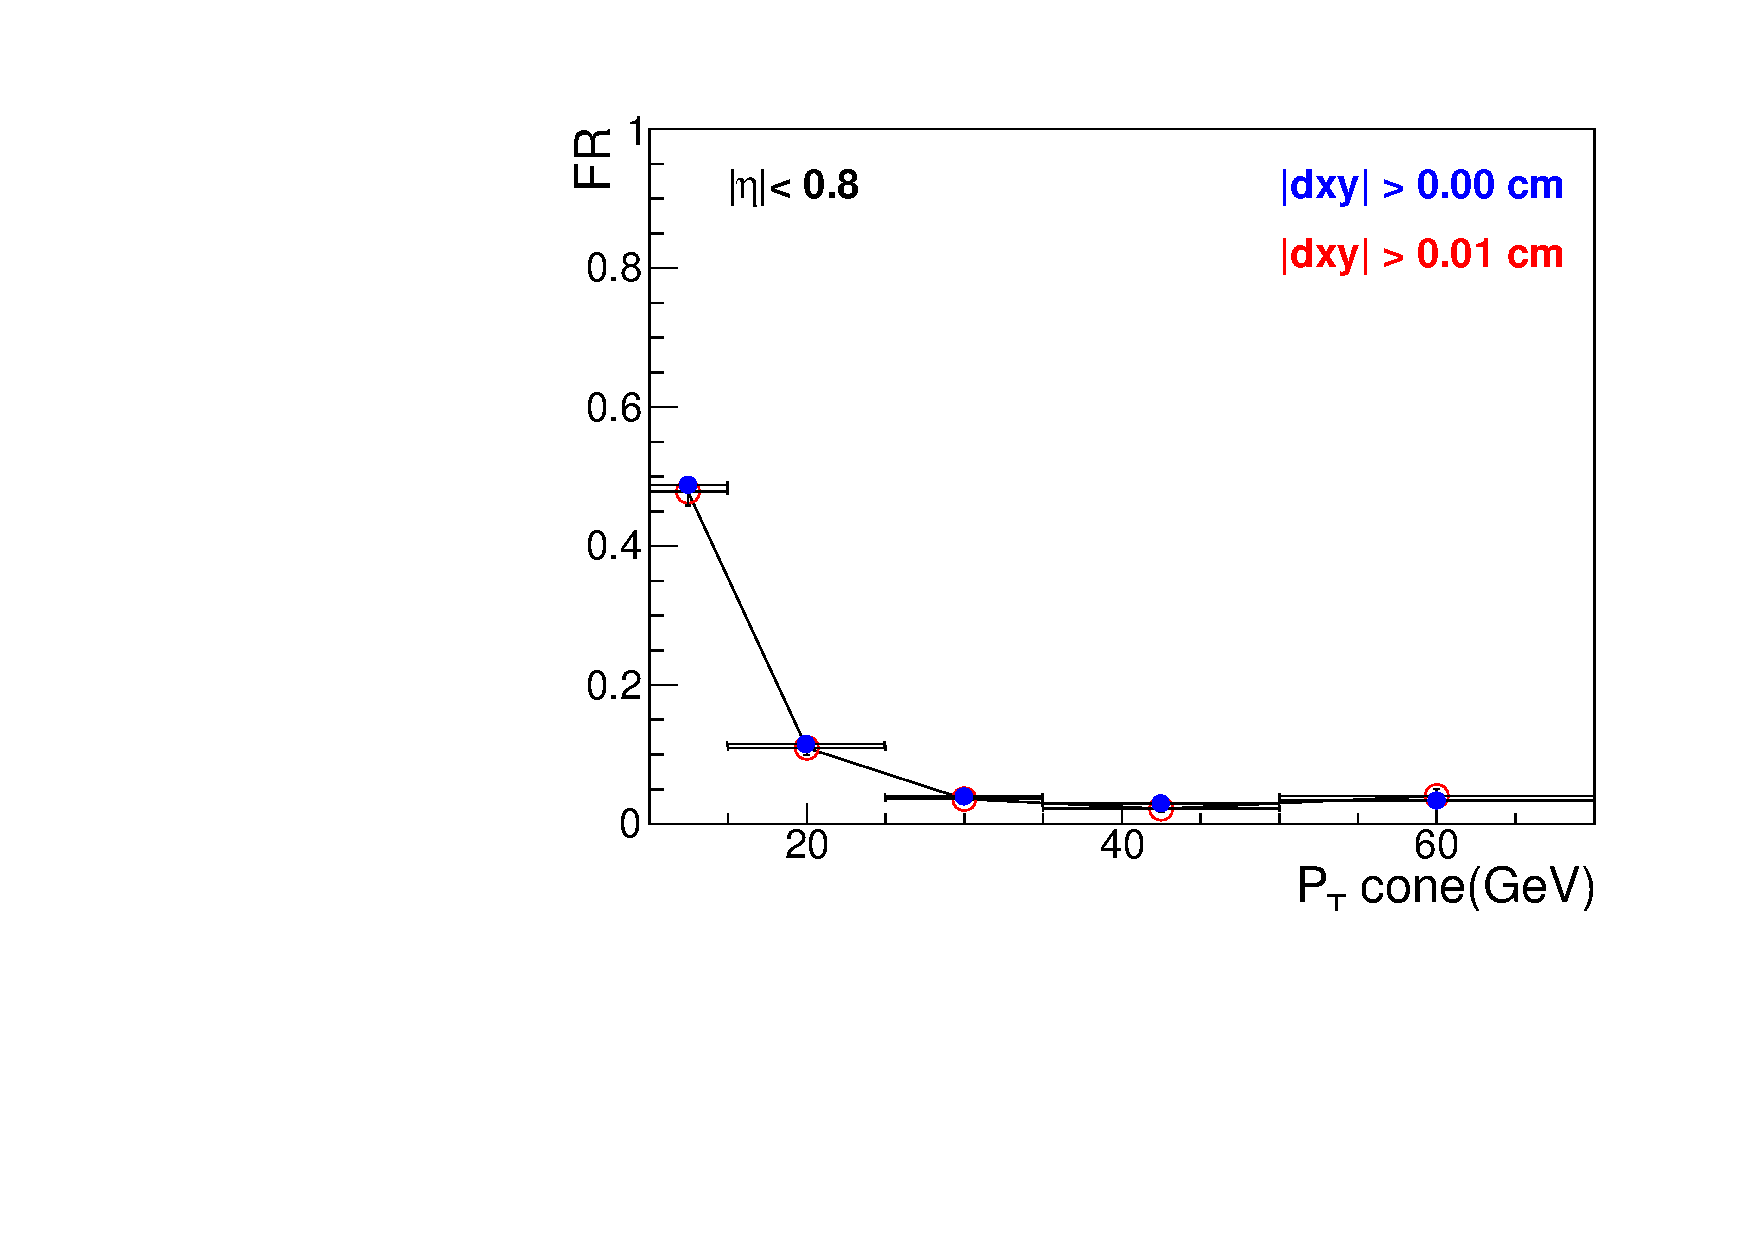
\includegraphics[width=.48\textwidth]{Figures/c6/backgrounds/FR/sFR/QCD/eta1_ele_dxy_comparison.pdf}
  \hfill{}
  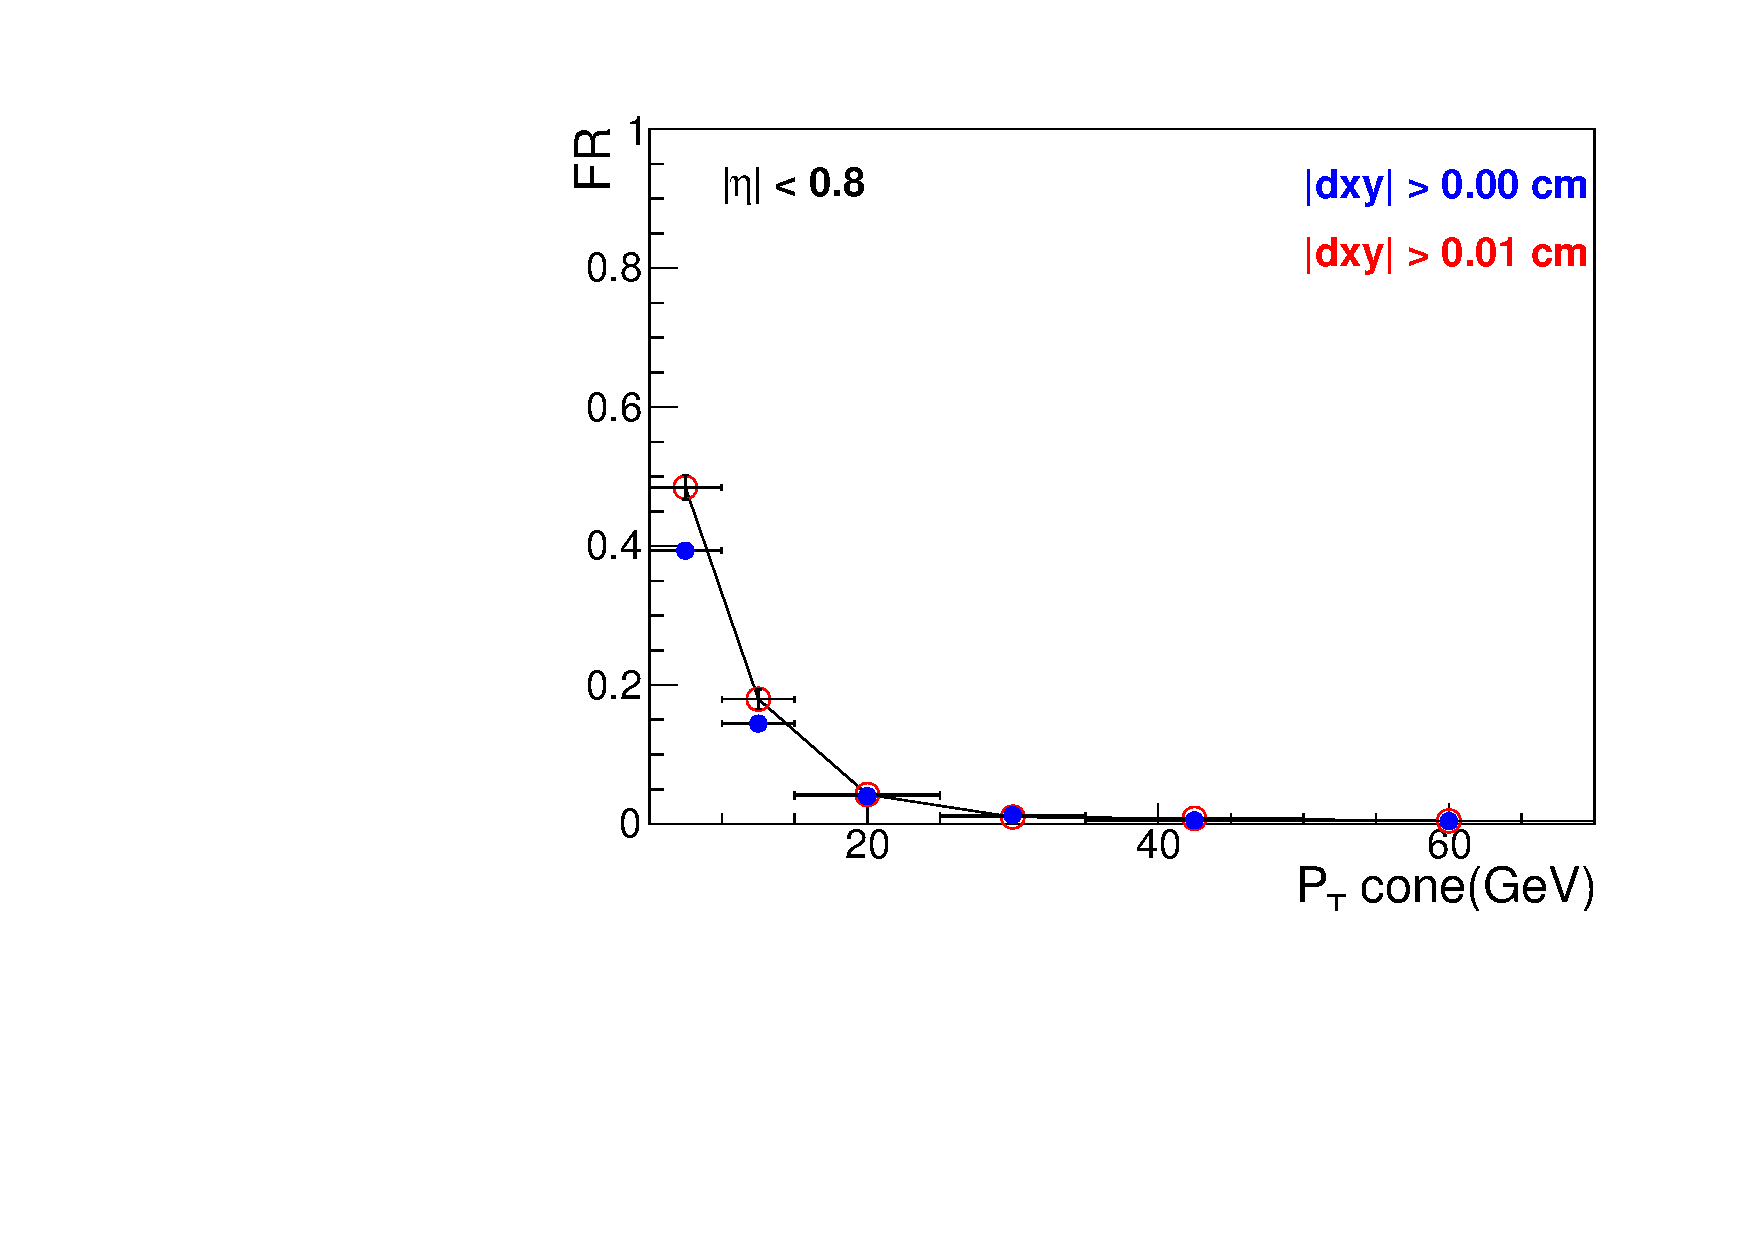
\includegraphics[width=.48\textwidth]{Figures/c6/backgrounds/FR/sFR/QCD/eta1_mu_dxy_comparison.pdf}\\
  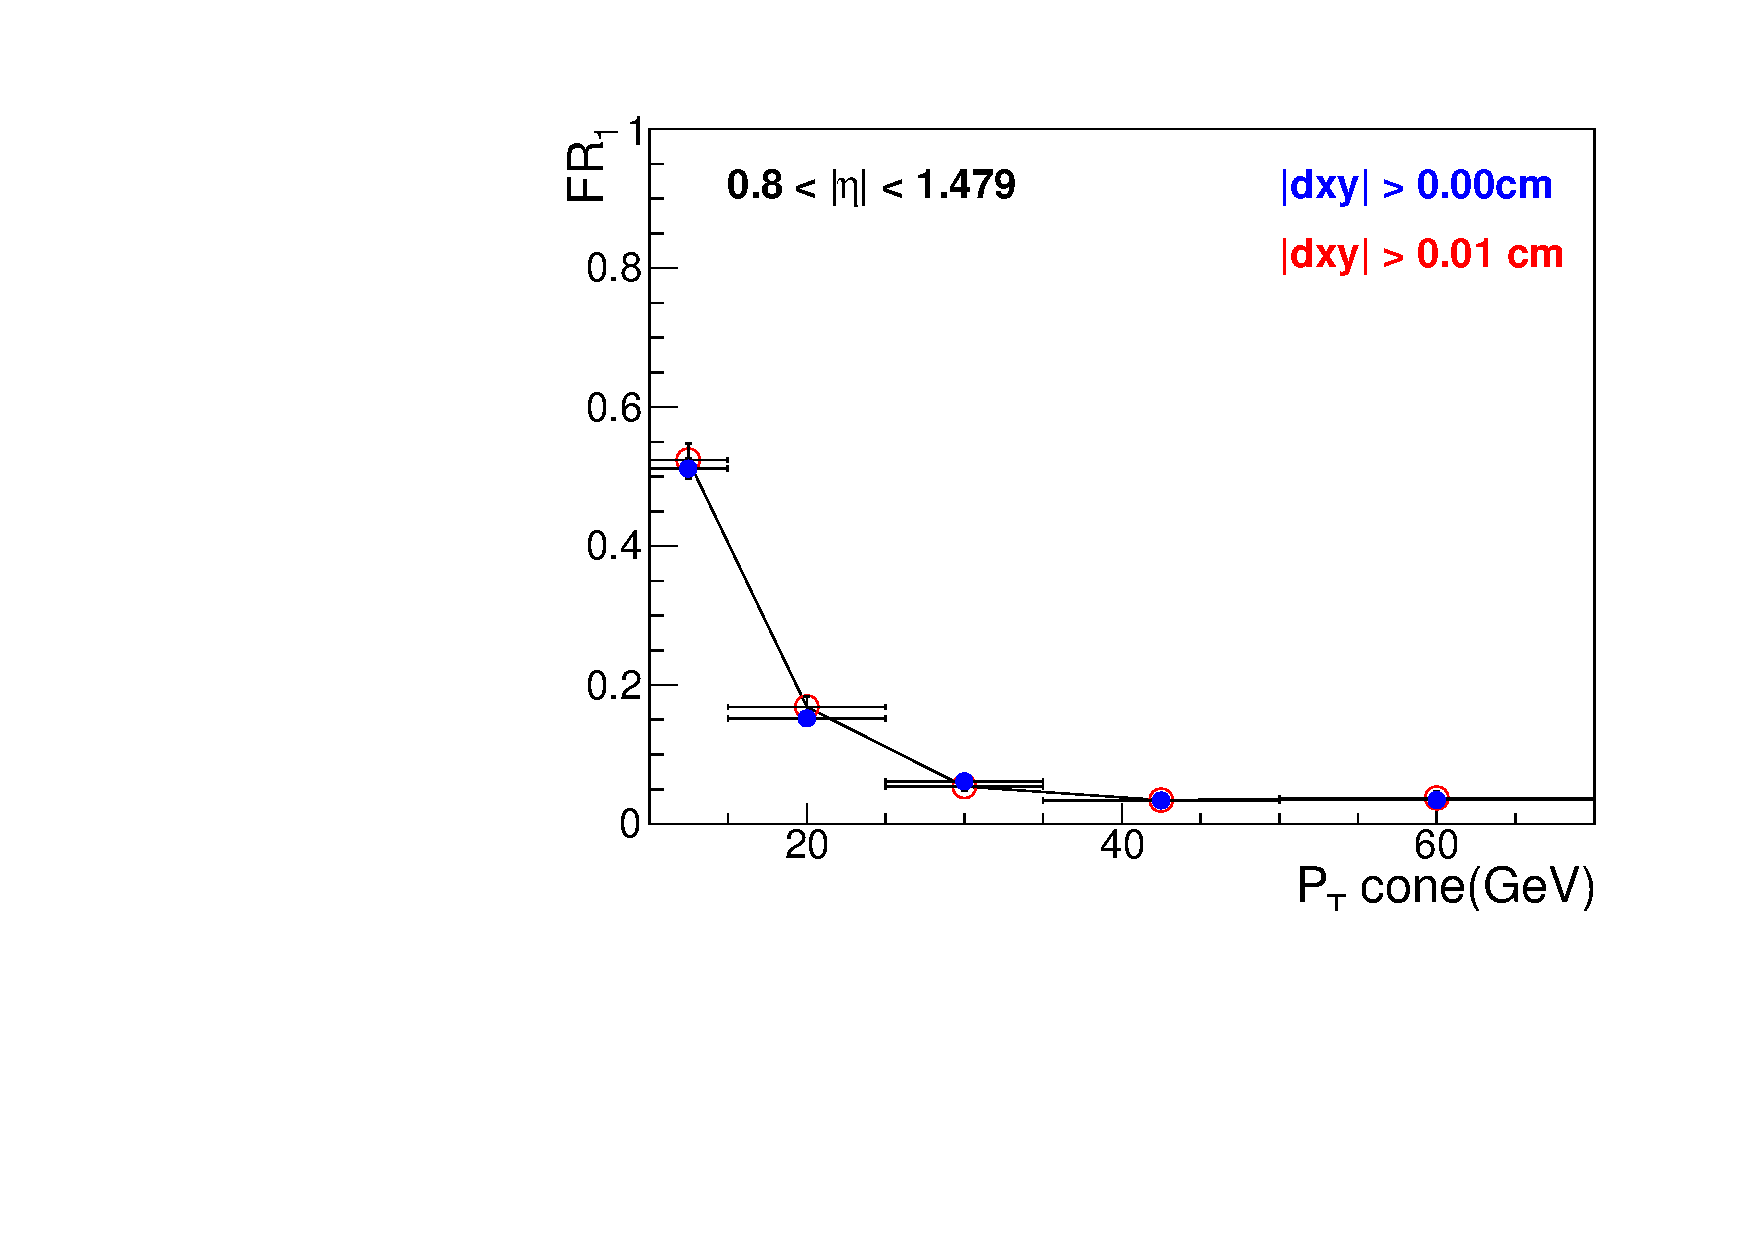
\includegraphics[width=.48\textwidth]{Figures/c6/backgrounds/FR/sFR/QCD/eta2_ele_dxy_comparison.pdf}
  \hfill{}
  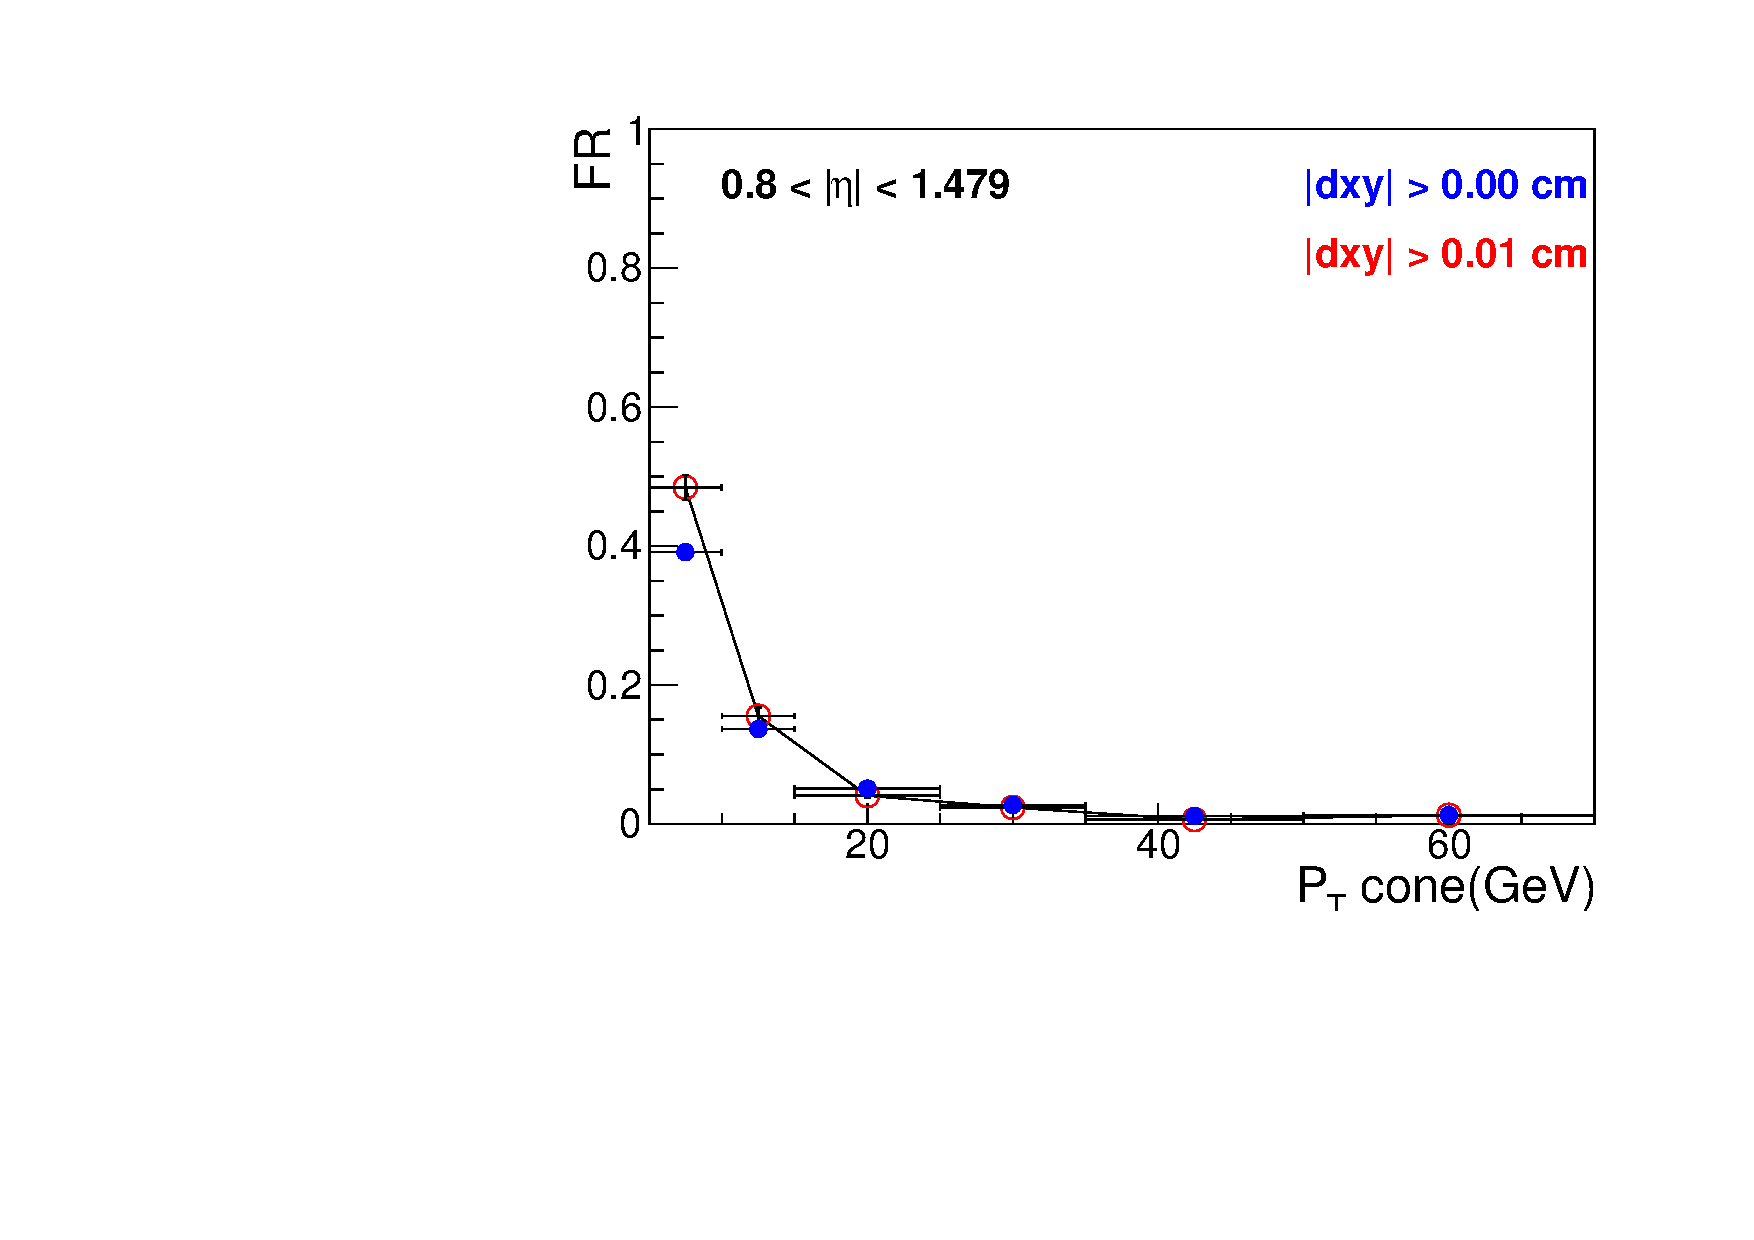
\includegraphics[width=.48\textwidth]{Figures/c6/backgrounds/FR/sFR/QCD/eta2_mu_dxy_comparison.pdf}\\
  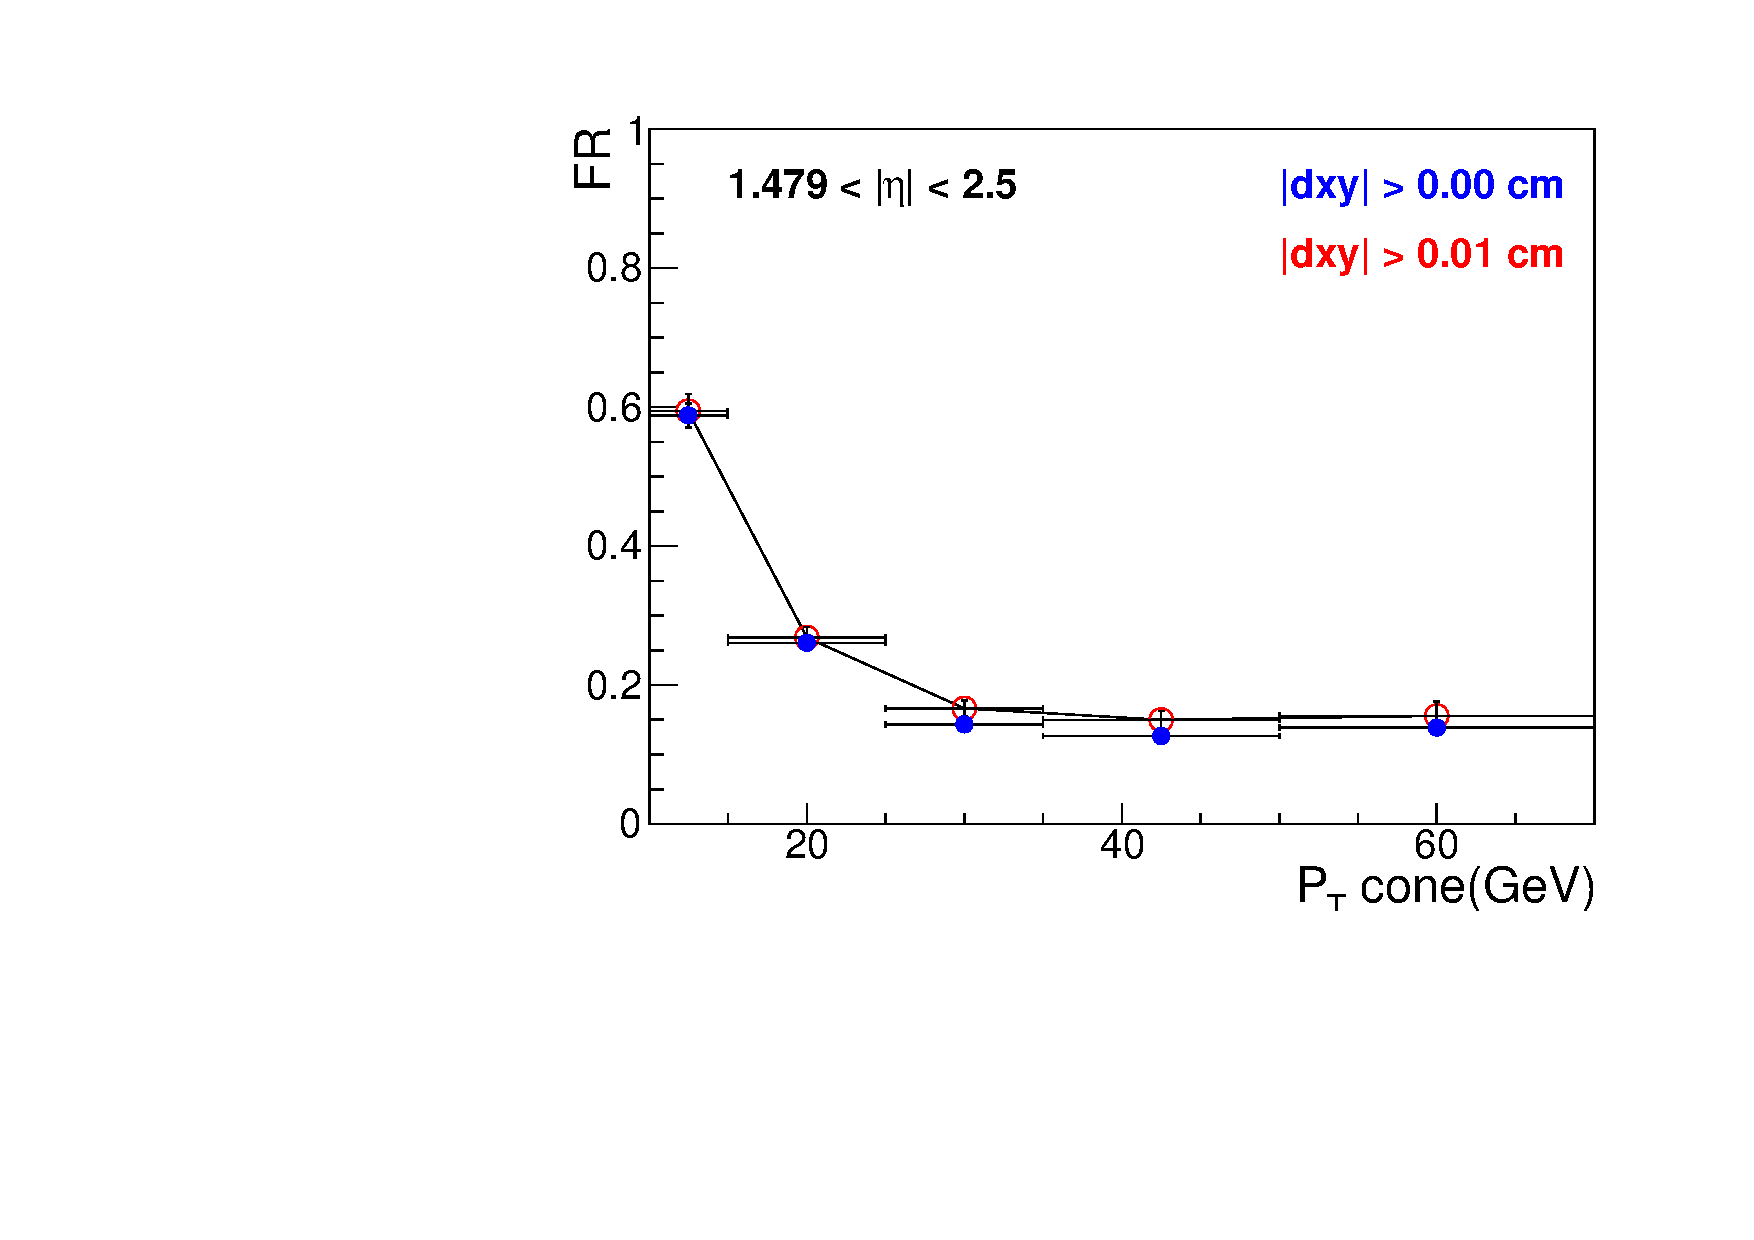
\includegraphics[width=.48\textwidth]{Figures/c6/backgrounds/FR/sFR/QCD/eta3_ele_dxy_comparison.pdf}
  \hfill{}
  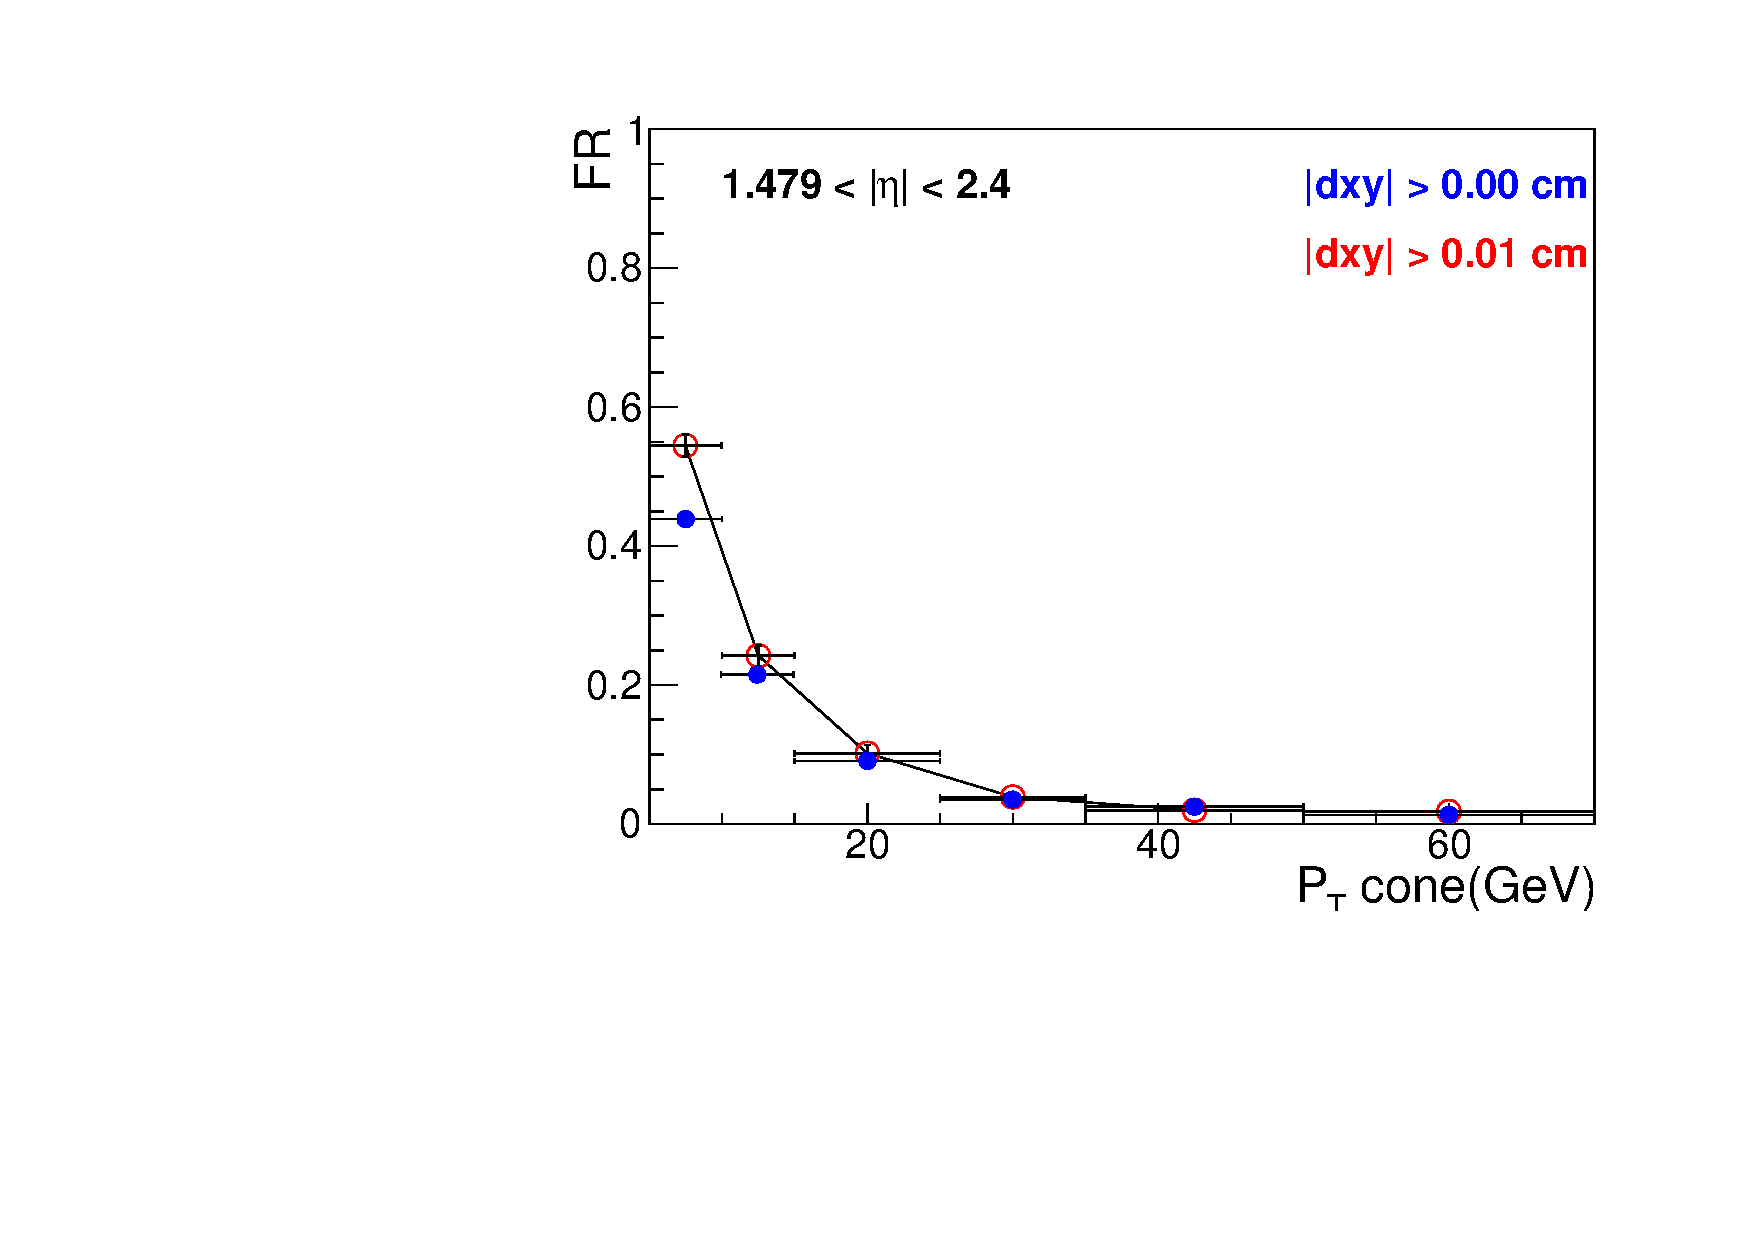
\includegraphics[width=.48\textwidth]{Figures/c6/backgrounds/FR/sFR/QCD/eta3_mu_dxy_comparison.pdf}
  \caption{Single fake rates obtained in 2016 simulation for electrons
    (left) and muons (right) as
    a function of \ptc, for \abseta ranges $[0,0.8]$ (top),
    $[0.8,1.479]$ (middle), and $[1.479,2.5]$ (bottom), calculated considering leptons with
    $\dxy> 0.01\cm$ (red) or with no \dxy contraints (blue).}
  \label{fig:sFR_dxy_comparison}
\end{figure}

The application region for single-fake lepton backgrounds (sFR)
is defined using the same selection as the signal region (see
Table~\ref{tab:baselinesel}), but with one (sFR$_1$) or two (sFR$_2$)
loose-not-tight nonprompt leptons that be not associated to the same
jet.
The background from single-fake leptons in the signal region is
estimated from the event yields in the application regions sFR using
the formula
\begin{linenomath}
  \begin{equation}
    \label{eq:sFRbkg}
    N_{\mathrm{sFR}}^{\mathrm{sig}} ~=~ 
    \sum_i\frac{\sfr(\sigeta_i,\,\ptcs{i})}{1-\sfr(\sigeta_i,\,\ptcs{i})}
    ~-~ 
    \sum_{j,\,k}\frac{\sfr(\sigeta_j,\,\ptcs{j})\,\sfr(\sigeta_k,\,\ptcs{k})}{\left(1-\sfr(\sigeta_j,\,\ptcs{j})\right)\left(1-\sfr(\sigeta_k,\,\ptcs{k})\right)}\;,
  \end{equation}
\end{linenomath}
where the first sum runs over all the events in sFR$_1$
(one loose-not-tight nonprompt lepton with pseudorapidity $\sigeta_i$
and transverse momentum \ptcs{i}),
while the sums in the second term run over the events in sFR$_2$
(two loose-not-tight nonprompt leptons with pseudorapidities
$\sigeta_j$ and $\sigeta_k$ and transverse momenta \ptcs{j} and
\ptcs{k}).
The minus sign in the second term is to remove the double counting due
to the contamination of sFR$_1$ events in the sFR$_2$ region.